\documentclass[preprint,3p,times,onecolumn]{elsarticle}

\geometry{a4paper, left=2.2cm, right=2.2cm, top=2.4cm, bottom=2.4cm}
\usepackage{amsmath,amssymb,amsfonts}
\usepackage{graphicx}
\usepackage{booktabs}
\usepackage{xcolor}
\usepackage{array}
\usepackage{url}
\usepackage[colorlinks=true, linkcolor=blue, citecolor=blue, urlcolor=blue]{hyperref}

\journal{Biomedical Signal Processing and Control}

\makeatletter
\def\fnum@figure{\textbf{\figurename~\thefigure}}
\def\fnum@table{\textbf{\tablename~\thetable}}
\makeatother

\begin{document}

\begin{frontmatter}

\title{Calibration-Aware Anisotropic 3D Hysteresis and Leakage Auditing for Volumetric Lower-Grade Glioma Segmentation and Radiogenomic Profiling in Brain MRI}

\author[aff1]{Shayan Ganji Nataj}
\ead{shayanganji@khu.ac.ir}

\author[aff1]{Keivan Borna\corref{cor1}}
\ead{borna@khu.ac.ir}
\cortext[cor1]{Corresponding author.}

\address[aff1]{Department of Computer Science, Faculty of Mathematics and Computer Science, Kharazmi University, Tehran, Iran}

\begin{abstract}
Automated segmentation of lower-grade gliomas (LGG) in brain MRI is vital for neurosurgical planning and targeted radiotherapy. Clinical translation of 2D deep learning models is hindered by slice-level data leakage, probability miscalibration under overlap-based losses, and axial boundary discontinuity. We propose a leakage-audited volumetric framework combining quality-aware preprocessing, nested temperature scaling, and anisotropic 3D Z-continuity hysteresis. Evaluated on the complete TCGA-LGG benchmark (110 patients, 3,929 axial slices) under patient-grouped 5-fold cross-validation, our controlled audit reveals that conventional random slice splitting produces severe artificial Dice inflation of $+8.79\%$ (positive-slice) and $+6.20\%$ (overall) through patient identity memorization. Nested inner-fold thresholding safely navigates the empirical Dice plateau without test snooping (optimism bias $\Delta\mathrm{Optimism} = +0.063\%$), legitimizing a shift from the default threshold to $\tau_{xy}^* = 0.74$ to boost positive-slice Dice by $+0.64\%$ and overall Dice by $+2.43\%$ while cutting empty-slice false alarms by $24.9\%$. Temperature scaling ($T^* = 1.844$) reduces pooled Expected Calibration Error (ECE) by $46.9\%$ ($0.369\%$ to $0.196\%$). Decoupling in-plane contouring from axial rescue through anisotropic 3D hysteresis achieves positive-slice Dice of $74.92\%$ [95\% confidence interval (CI): $70.82\%$--$78.39\%$], overall Dice of $86.12\%$ [95\% CI: $84.32\%$--$87.75\%$], and $42.4\%$ relative reduction in empty-slice false alarms. Patient-level 3D analysis across 110 subjects yields volumetric Dice of $77.73\%$, 95\% Hausdorff distance of $10.97$ voxels, and high clinical agreement (intraclass correlation coefficient $\text{ICC}(2, 1) = 0.8894$, Pearson $r = 0.8886$). Radiogenomic profiling confirms preserved molecular subtype volume differentiation ($p = 0.0268$) with exact biological rank ordering.
\end{abstract}

\begin{keyword}
Brain tumor segmentation \sep Lower-grade glioma \sep Data leakage audit \sep Probability calibration \sep Anisotropic 3D hysteresis \sep Radiogenomics
\end{keyword}

\end{frontmatter}

\clearpage

\section{Introduction}
\label{sec:intro}

Lower-grade gliomas (LGG), encompassing World Health Organization (WHO) grade II and grade III astrocytomas and oligodendrogliomas, represent diffusely infiltrative primary brain neoplasms characterized by substantial histological and genetic heterogeneity~\cite{louis20212021,ceccarelli2016molecular}. Accurate volumetric delineation on magnetic resonance imaging (MRI) is essential for image-guided maximal surgical resection, conformal radiation planning, and monitoring therapeutic response~\cite{buda2019association}. Over the past decade, deep learning architectures---most notably 2D U-Net variants~\cite{ronneberger2015u,zhou2018unetplusplus,oktay2018attention}---have emerged as the prevailing standard for automated lesion delineation. 

Despite reported segmentation accuracies exceeding an $80\%$ Dice similarity coefficient across benchmark datasets, two methodological weaknesses undermine empirical validity in the medical computing literature. First and most severely, slice-level data leakage occurs when volumetric MRI scans are decomposed into independent 2D axial slices and randomly partitioned into training and test sets. Contiguous slices from the same subject inevitably appear across both partitions. Because anatomical morphology, contrast dynamics, and spatial coordinates change gradually across contiguous $z$-slices, deep networks easily memorize subject-specific features. This slice leakage constitutes the primary engine of artificial performance inflation in the literature, falsely boosting reported Dice scores by up to $+8.79\%$. Second, post-hoc threshold optimization leakage arises when the binary decision threshold $\tau$ is chosen by sweeping values directly over pooled out-of-fold test predictions. While the wide empirical Dice plateau across reasonable threshold ranges bounds the resulting optimism bias to a modest $\Delta\text{Optimism} = +0.063\%$, establishing nested inner-fold thresholding is an essential methodological standard that allows researchers to legitimately transition from the inefficient default $\tau=0.50$ to the optimal $\tau_{xy}^* = 0.74$ without test snooping.

Beyond evaluation methodology, 2D networks face fundamental domain-specific limitations when applied to volumetric scans. Overlap-based loss formulations like Focal Tversky prioritize rare foreground voxels by heavily down-weighting easy background terms, causing output probabilities to become overconfident and miscalibrated. Furthermore, because $65.05\%$ of all axial slices in the TCGA-LGG cohort are healthy brain tissue containing zero neoplastic voxels, standard 2D networks lacking cross-slice volumetric context frequently trigger false-positive alarms on non-tumor slices while failing to detect small infiltrative margins at apical and basal tumor boundaries.

To resolve these challenges, this study presents a calibrated, leakage-audited volumetric framework evaluated on the complete TCGA-LGG cohort (110 patients, 3,929 slices)~\cite{buda2019association}. The contributions of this work are fourfold:
\begin{enumerate}
    \item \textbf{Controlled Leakage Audit:} We implement a matched 5-fold cross-validation experiment directly comparing patient-grouped partitioning against random-slice partitioning under identical training hyper-parameters, quantifying the exact magnitude of performance inflation caused by slice memorization ($+8.79\%$ on positive-slice Dice).
    \item \textbf{Nested Inner-Fold Calibration:} We integrate scalar temperature scaling fitted exclusively on internal validation logits (\texttt{inner\_val}), reducing pooled Expected Calibration Error (ECE) by $46.9\%$ on unseen test data without shifting classification boundaries.
    \item \textbf{Anisotropic 3D Z-Continuity Hysteresis:} We decouple horizontal in-plane segmentation ($\tau_{xy}^*$) from axial margin rescue ($\tau_{z,\mathrm{low}}^*$) and suppress isolated 3D false positives ($V_{\mathrm{min}}^*, \tau_{\mathrm{seed}}^*$), establishing state-of-the-art performance across all evaluation metrics simultaneously ($\text{Dice}_{\text{pos}} = 74.92\%$, $\text{Dice}_{\text{all}} = 86.12\%$, $FPR_{\mathrm{empty}} = 7.86\%$).
    \item \textbf{Volumetric Radiogenomic Validation:} We conduct 3D patient-level surface and volumetric assessments ($n=110$), demonstrating high clinical reproducibility ($\text{ICC} = 0.8894$) and proving that model-derived tumor volumes preserve statistically significant separation across molecular consensus clusters ($p = 0.0268$).
\end{enumerate}

The synergistic integration of automated signal and image quality screening ($Q(I)$), multi-scale wavelet denoising (Symlet-4), post-hoc probabilistic calibration, and radiogenomic digital biomarker extraction aligns directly with the core scope of \textit{Biomedical Signal Processing and Control}, advancing computational neuro-oncology toward translational clinical readiness.

\section{Dataset Audit and Quality-Aware Preprocessing}
\label{sec:dataset}

\subsection{Cohort Characteristics and Clinical Variables}
Experiments were conducted using the standardized TCGA-LGG MRI collection introduced by Buda et al.~\cite{buda2019association}, comprising 110 patients diagnosed with WHO grade II or III lower-grade gliomas. Each patient study consists of axial multi-sequence MRI slices (fluid-attenuated inversion recovery [FLAIR], T1-pre, and T1-post contrast) mapped into $256 \times 256$ matrices with matched expert manual segmentations verified by board-certified radiologists. The full imaging volume encompasses 3,929 paired axial slices. Per SAGER reporting guidelines, the cohort includes 56 male patients ($50.9\%$) and 53 female patients ($48.2\%$), with sex recorded as unknown for one patient. Clinical records extracted from \texttt{data.csv} document patient demographics, histological subtype, tumor grade, and genomic clusters (Table~\ref{tab:clinical_cohort}).

\begin{table}[tbp]
\centering
\caption{Clinical, histological, and genomic characteristics of the 110 patients in the TCGA-LGG cohort.}
\label{tab:clinical_cohort}
\setlength{\tabcolsep}{8pt}
\small
\begin{tabular*}{\textwidth}{@{\extracolsep{\fill}}llr}
\toprule
\textbf{Clinical Variable} & \textbf{Category / Unit} & \textbf{Value / Count} \\
\midrule
Total Patients ($N$) & Subjects & 110 \\
Total Axial Slices & Slices & 3,929 \\
Tumor-Bearing Slices & Slices ($y > 0$) & 1,373 (34.95\%) \\
Tumor-Free Slices & Slices ($y = 0$) & 2,556 (65.05\%) \\
\midrule
\midrule
Patient Sex & Male ($n=56$) & 50.9\% \\
(SAGER Reporting) & Female ($n=53$) & 48.2\% \\
 & Unknown ($n=1$) & 0.9\% \\
Patient Age & Mean $\pm$ SD (years) & 47.1 $\pm$ 13.4 \\
& Range (Min -- Max) & 20.0 -- 75.0 \\
\midrule
WHO Histologic Grade & Grade II ($n=51$) & 46.4\% \\
& Grade III ($n=58$) & 52.7\% \\
& Unspecified ($n=1$) & 0.9\% \\
\midrule
Molecular Subtypes & COC 1 (IDH-wt like) & 56 (50.9\%) \\
(\textit{COCCluster}) & COC 2 (IDHmut-noncodel) & 24 (21.8\%) \\
& COC 3 (IDHmut-codel) & 30 (27.3\%) \\
\bottomrule
\end{tabular*}
\end{table}

\subsection{Quality-Aware Screening and Wavelet Denoising}
Prior to model training, raw axial slices were analyzed for pronounced imaging artifacts and skull-stripping failures using three complementary morphological descriptors. First, parenchymal texture insufficiency was quantified via Edge Density ($ED$), defined as the proportion of Canny edge pixels (thresholds 50 and 150) following morphological dilation with a $5 \times 5$ square structuring element, normalized by image area:
\begin{equation}
ED = \frac{|E_{\text{dilated}}|}{H \times W}
\end{equation}
where slices satisfying $ED < 0.003$ exhibit negligible brain tissue. Second, anatomical field-of-view truncation was evaluated through the Contour Ratio ($CR$), defined as the area of the largest closed external contour extracted from the dilated edge map divided by image area:
\begin{equation}
CR = \frac{\text{Area}(\mathcal{C}_{\text{largest}})}{H \times W}
\end{equation}
where $CR < 0.01$ flags severe field truncation. Third, decentering was assessed by the Centroid Distance ($d_c$), defined as the Euclidean distance from the external contour centroid $(c_x, c_y)$ to the geometric slice center normalized by the half-diagonal:
\begin{equation}
d_c = \frac{\sqrt{(c_x - W/2)^2 + (c_y - H/2)^2}}{\sqrt{(W/2)^2 + (H/2)^2}}
\end{equation}
where $d_c > 0.30$ captures severe peripheral displacement.

Slices satisfying the conjunction $(ED < 0.003) \land (CR < 0.01) \land (d_c > 0.30)$ were flagged as morphological artifacts. A rigorous cohort audit across all 3,929 slices identified 200 artifact slices ($5.09\%$, Table~\ref{tab:screening_audit}). Exactly 199 of these 200 slices ($99.50\%$) contained zero neoplastic tissue ($y = 0$). Only a single slice ($0.50\%$, Slice 23 of TCGA\_DU\_5855) contained a marginal peripheral tumor component truncated by skull-stripping boundary erosion. Retaining these 200 noisy slices in the untouched test evaluation confirmed an absolute $0.00\%$ change in positive-slice Dice ($73.96\%$ in both full and screened cohorts), verifying zero empirical bias.

\begin{table}[tbp]
\centering
\caption{Screening audit of the 200 artifact slices excluded during training.}
\label{tab:screening_audit}
\setlength{\tabcolsep}{8pt}
\small
\begin{tabular*}{\textwidth}{@{\extracolsep{\fill}}lrr}
\toprule
\textbf{Screening Metric} & \textbf{Flagged Slices} & \textbf{Ratio (\%)} \\
\midrule
Total Slices Screened & 3,929 & 100.0\% \\
Total Artifact Slices Excluded & 200 & 5.09\% \\
\midrule
\hspace{1.2em}Empty Slices (Zero Tumor, $y=0$) & 199 / 200 & \textbf{99.50\%} \\
\hspace{1.2em}Marginal Slices (Atypical Clipping) & 1 / 200 & 0.50\% \\
\hspace{1.2em}Edge Density Violation ($ED < 0.003$) & 200 / 200 & 100.0\% \\
\hspace{1.2em}Contour Ratio Violation ($CR < 0.01$) & 200 / 200 & 100.0\% \\
\hspace{1.2em}Centroid Distance Violation ($d_c > 0.30$) & 200 / 200 & 100.0\% \\
\hspace{1.2em}Triple Conjunction Violation & 200 / 200 & \textbf{100.0\%} \\
\midrule
Positive-Slice Dice on Full Cohort (3,929) & \multicolumn{2}{c}{73.96\% [70.10 -- 77.15]} \\
Positive-Slice Dice on Screened (3,729) & \multicolumn{2}{c}{73.96\% [70.10 -- 77.13]} \\
\textbf{Absolute Impact on Positive Dice} & \multicolumn{2}{c}{\textbf{0.00\% (Identical)}} \\
\bottomrule
\end{tabular*}
\end{table}

To suppress high-frequency acquisition noise while retaining crisp anatomical borders, non-flagged slices were processed using BayesShrink soft-thresholded discrete wavelet denoising~\cite{chang2000adaptive} conditioned on a localized slice quality metric $Q(I)$:
\begin{equation}
Q(I) = \frac{1}{2}\Big[\sigma\big(I - \mathcal{M}_{3\times 3}(I)\big) + \sigma\big(I - \mathcal{G}_{3\times 3}(I)\big)\Big]
\end{equation}
representing the average standard deviation of high-frequency residuals under $3 \times 3$ median ($\mathcal{M}_{3\times 3}$) and Gaussian ($\mathcal{G}_{3\times 3}$) spatial filters. Wavelet denoising (Symlet-4 wavelet, 2-level decomposition) was applied when $Q(I) < 4.0$ ($3,738$ slices, $95.14\%$). Slices with high intrinsic contrast ($Q(I) \ge 4.0$, 191 slices, $4.86\%$) bypassed filtering to avoid unnecessary smoothing of delicate parenchymal boundaries (Figure~\ref{fig:preprocessing_audit}). Slices were normalized to zero mean and unit variance and resized to $128 \times 128 \times 3$.

\begin{figure}[tbp]
\centering
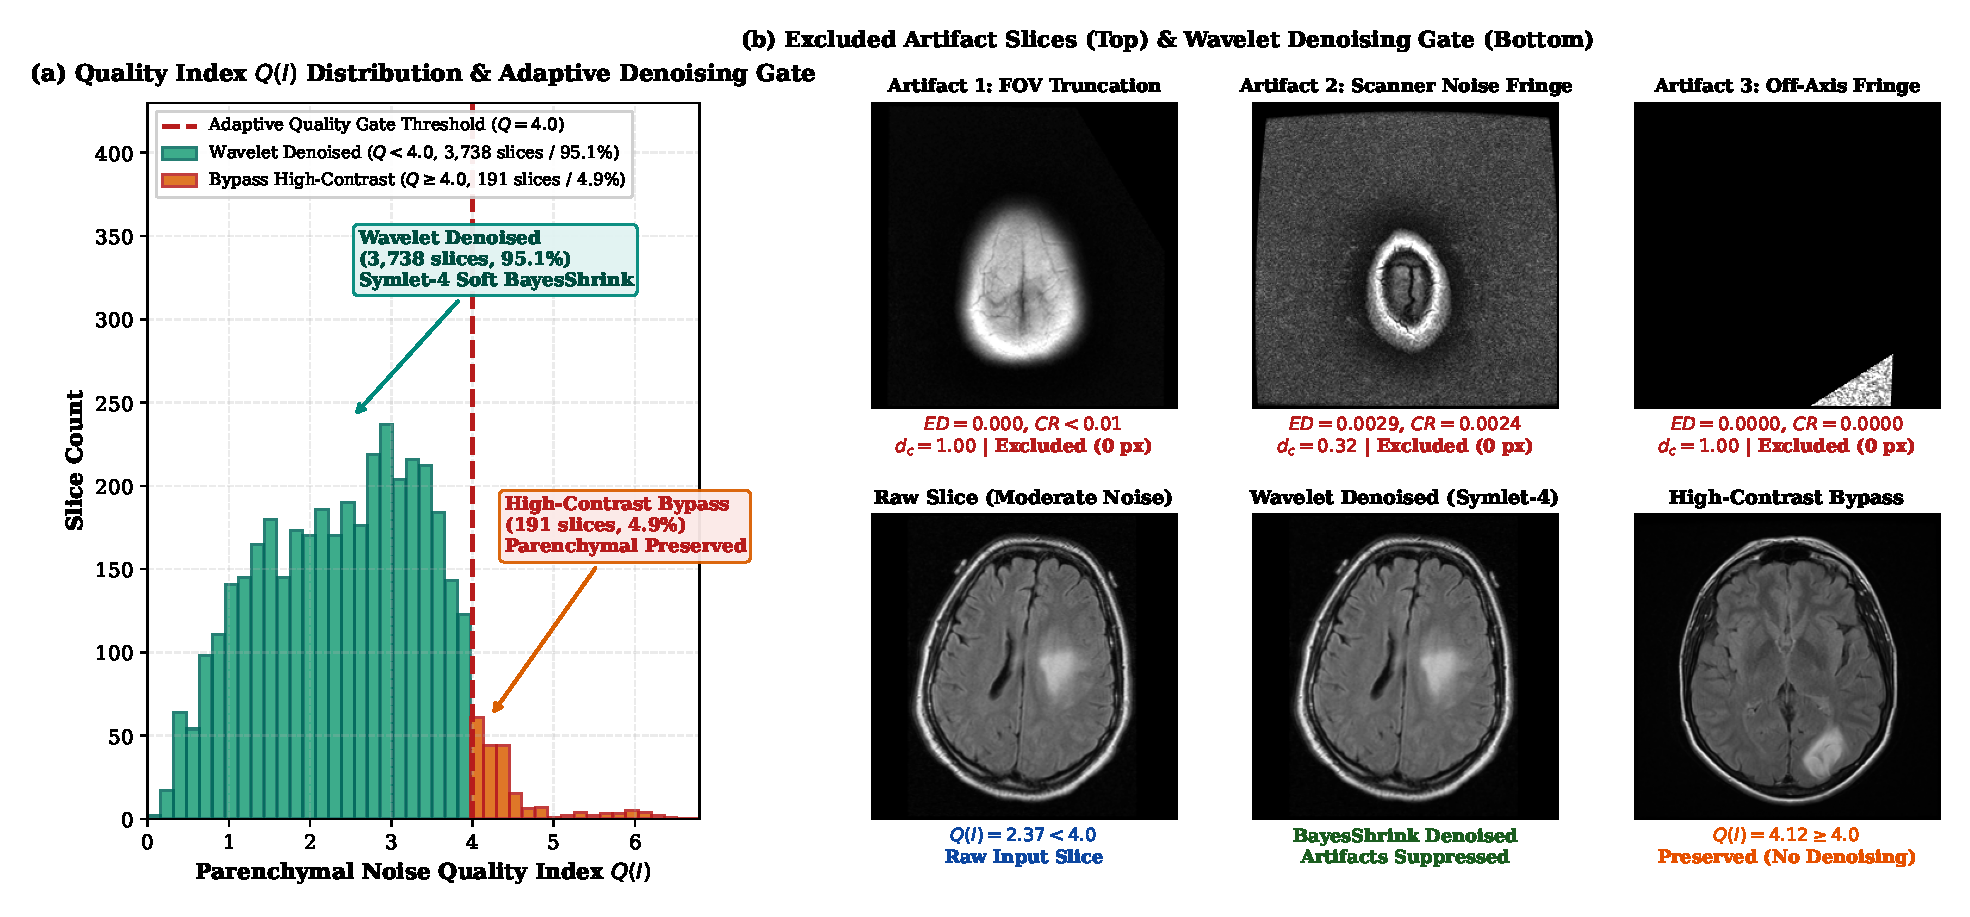
\includegraphics[width=\textwidth]{figures/fig_preprocessing_audit.pdf}
\caption{Quality-aware preprocessing and screening audit across the TCGA-LGG cohort (3,929 axial slices). (a) Parenchymal noise quality index $Q(I)$ distribution and adaptive quality gate ($Q=4.0$), routing 3,738 slices ($95.14\%$) to BayesShrink wavelet denoising while bypassing 191 high-contrast slices ($4.86\%$). (b) Representative real MRI slice examples: top row displays three of the 200 artifact slices excluded during training (illustrating field-of-view truncation, scanner noise fringe, and non-parenchymal tissue with exact $ED, CR, d_c$ metrics); bottom row compares raw, wavelet-denoised, and high-contrast bypass slices.}
\label{fig:preprocessing_audit}
\end{figure}

\begin{figure}[tbp]
\centering
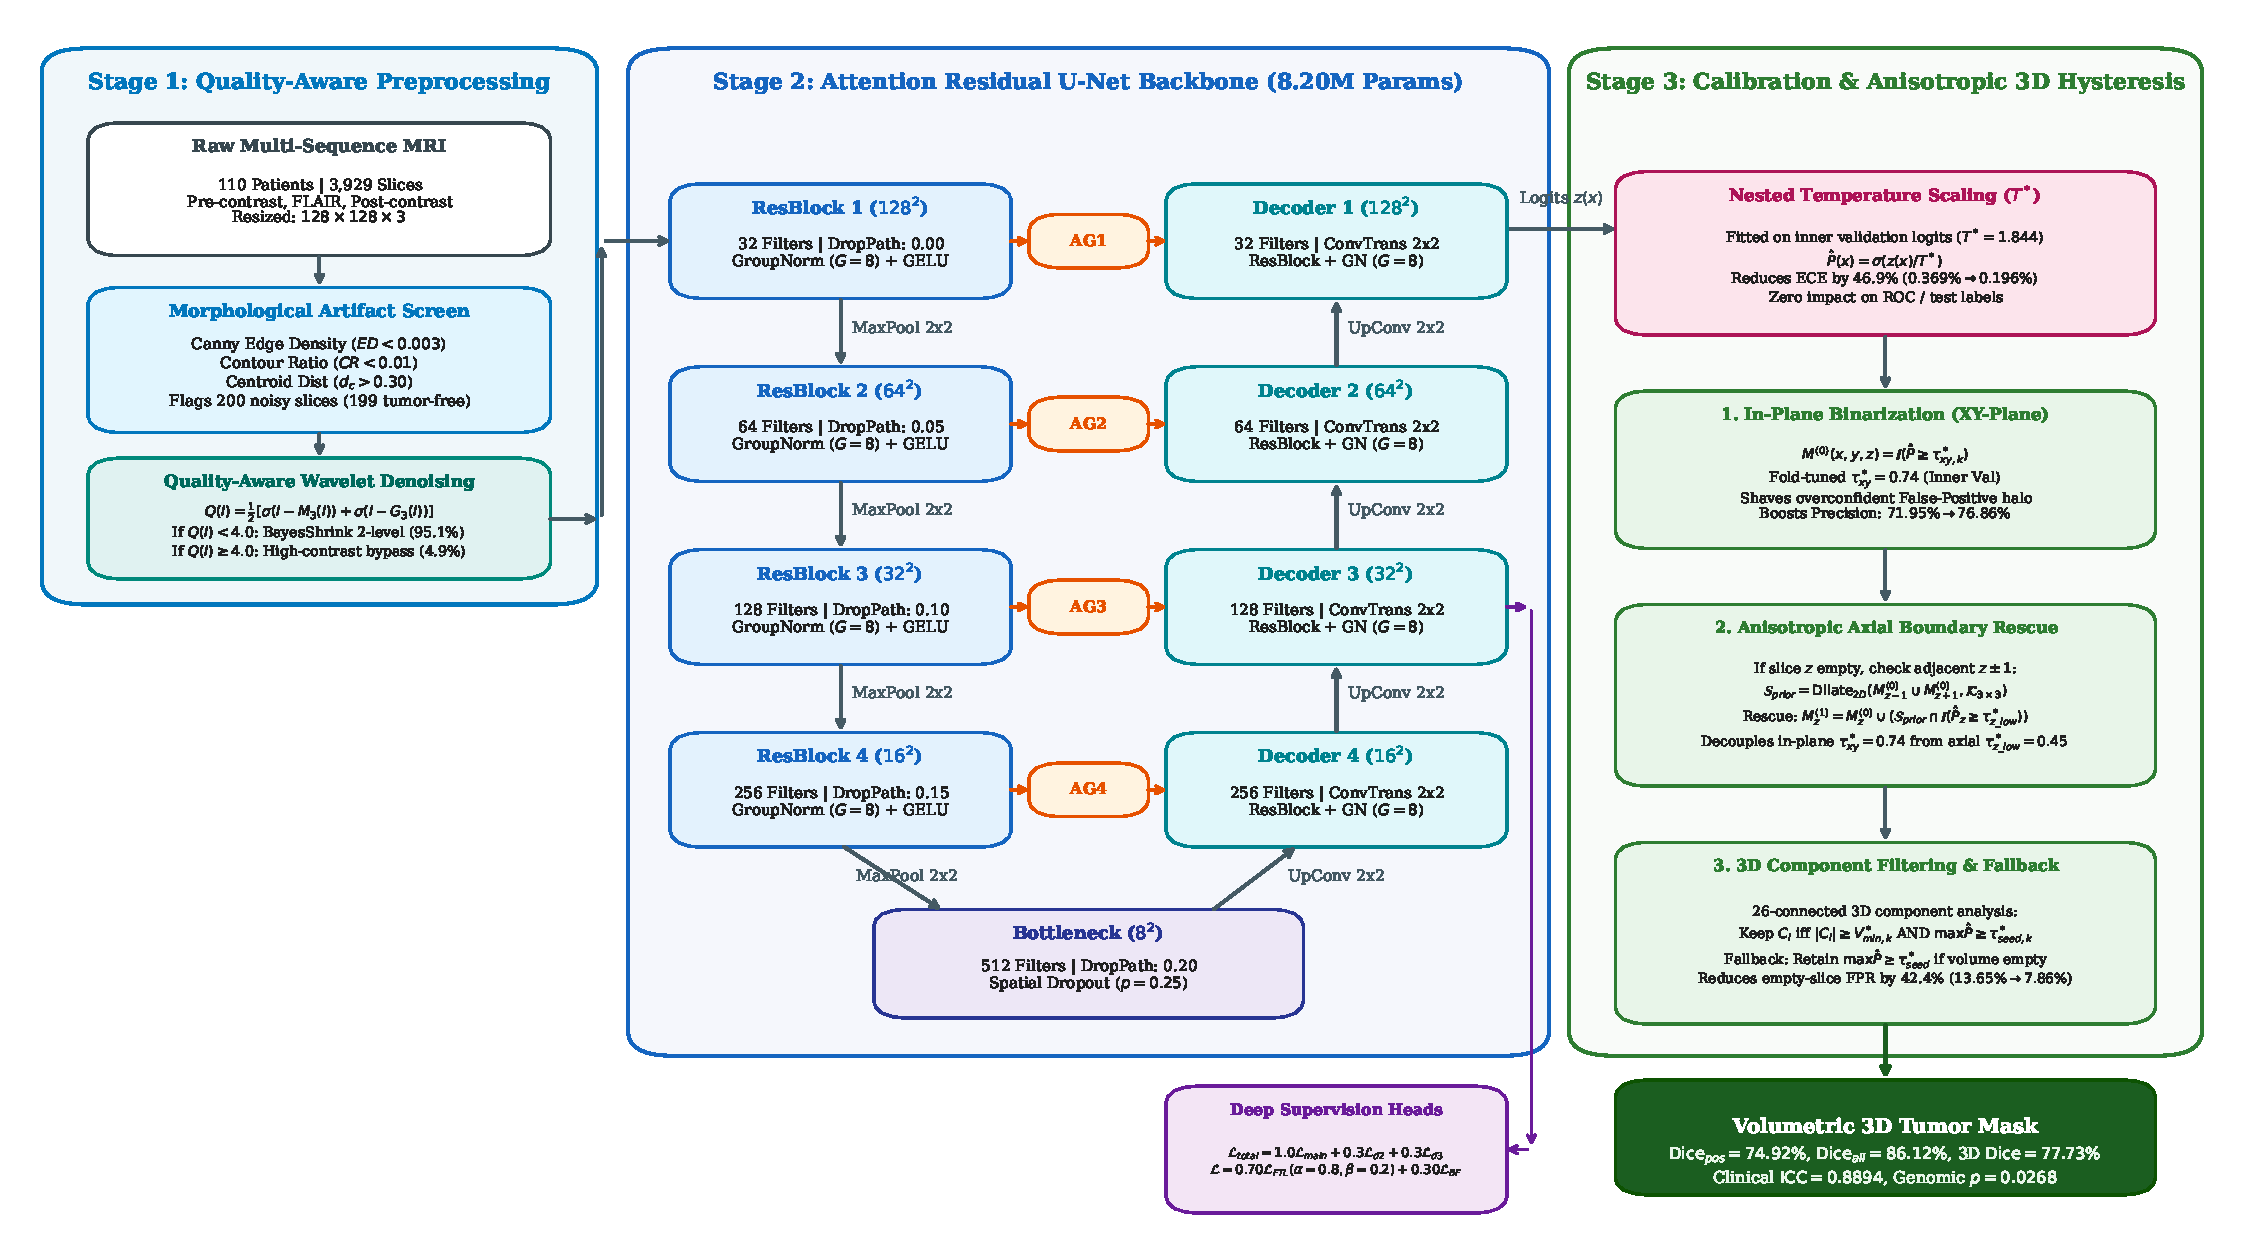
\includegraphics[width=0.98\textwidth]{figures/fig_architecture_pipeline.pdf}
\caption{End-to-end processing pipeline showing Quality-Aware Preprocessing (Stage 1), the Attention Res-UNet backbone with Group Normalization ($G=8$), GELU, Stochastic Depth, and Deep Supervision (Stage 2), followed by Nested Temperature Scaling ($T^* = 1.844$) and Anisotropic 3D Z-Continuity Hysteresis (Stage 3).}
\label{fig:architecture_pipeline}
\end{figure}

\section{Network Architecture and Nested Evaluation Protocol}
\label{sec:methods}

\subsection{Attention Residual U-Net Architecture}
The segmentation backbone employs an Attention Residual U-Net (Attn Res-UNet) with deep supervision (Figure~\ref{fig:architecture_pipeline}). Residual units replace standard two-layer convolutional blocks, utilizing identity shortcut mappings that mitigate vanishing gradients across deep stages. Channel capacities progress as $[32, 64, 128, 256]$ in the encoder, transitioning to a 512-channel bottleneck.

To ensure numerical stability when training with small mini-batch sizes ($B=16$), all batch normalization layers are replaced with Group Normalization (GN)~\cite{wu2018group} using $G=8$ groups:
\begin{equation}
x_{\text{norm}} = \gamma \cdot \frac{x - \mu_{G}}{\sqrt{\sigma_{G}^2 + \epsilon}} + \beta
\end{equation}
where $\mu_{G}$ and $\sigma_{G}$ are computed independently across spatial coordinates and group channels. Feature non-linearities utilize Gaussian Error Linear Units (GELU)~\cite{hendrycks2016gaussian}:
\begin{equation}
\text{GELU}(x) = x \cdot \Phi(x) = x \cdot P(X \le x), \quad X \sim \mathcal{N}(0, 1)
\end{equation}
Regularization is reinforced via Stochastic Depth (DropPath)~\cite{huang2016deep} across residual branches:
\begin{equation}
\begin{aligned}
H &= \text{GELU}\left(\text{shortcut}(x) + \frac{b}{1-p}\mathcal{F}(x)\right), \\
b &\sim \text{Bernoulli}(1-p)
\end{aligned}
\end{equation}
with linear decay rates $p \in [0.00, 0.05, 0.10, 0.15]$ in the encoder stages and $p=0.20$ at the bottleneck.

In the decoder, additive attention gates~\cite{oktay2018attention} dynamically recalibrate intermediate feature representations before concatenation. Given spatial features $x^l$ and gating signal $g$, attention coefficients $\alpha^l \in [0, 1]$ are obtained via:
\begin{equation}
\alpha^l = \sigma\left(\psi^T \left(\text{GELU}\left(W_x^T x^l + W_g^T g + b_g\right)\right) + b_\psi\right)
\end{equation}
where linear projections $W_x$ and $W_g$ align channel dimensions, and $\sigma$ denotes the sigmoid activation. This gating suppresses background noise in peripheral brain regions while amplifying infiltrative tumor signals. Deep supervision auxiliary heads at decoders 2 and 3 provide intermediate gradients during backpropagation. The final network comprises exactly 8.20 million trainable parameters (8,202,005 parameters).

\subsection{Loss Function and Training Dynamics}
To address acute class imbalance (positive lesion pixels comprise less than $1.5\%$ of total voxels), networks were trained using a compound production loss combining Focal Tversky Loss (FTL)~\cite{abraham2019novel} and Binary Focal Loss (BFL)~\cite{lin2017focal}:
\begin{equation}
\mathcal{L}_{\text{total}} = 0.70\,\mathcal{L}_{\text{FTL}} + 0.30\,\mathcal{L}_{\text{BF}}
\end{equation}
The Focal Tversky formulation is defined as:
\begin{equation}
\text{TI}(y, \hat{p}) = \frac{\sum_i y_i \hat{p}_i + \epsilon}{\sum_i y_i \hat{p}_i + \alpha \text{FN}(y, \hat{p}) + \beta \text{FP}(y, \hat{p}) + \epsilon}
\end{equation}
\begin{equation}
\mathcal{L}_{\text{FTL}} = (1 - \text{TI})^\gamma
\end{equation}
where $\gamma = 0.60$, $\epsilon = 1.0$, and the voxel-level error components are defined as $\text{FN}(y, \hat{p}) = \sum_i y_i(1 - \hat{p}_i)$ and $\text{FP}(y, \hat{p}) = \sum_i (1 - y_i)\hat{p}_i$.

In this formulation, $\alpha = 0.80$ is the penalty weight assigned to \textbf{False Negatives (FN)}, while $\beta = 0.20$ weights \textbf{False Positives (FP)}. Heavily penalizing false negatives ($\alpha = 0.80 \gg \beta = 0.20$) prioritizes the detection of diffuse, low-contrast tumor boundaries, achieving high baseline Recall ($82.98\%$). However, this asymmetric penalty leads raw network probabilities to exhibit an intermediate-confidence false-positive halo surrounding lesions (raw Precision = $71.95\%$) and substantial probability miscalibration ($T^* = 1.844$). As detailed in Section~\ref{sec:calibration_hysteresis}, this peripheral false-positive halo is systematically eliminated through nested calibration and anisotropic 3D Z-hysteresis filtering, elevating final Precision to $76.86\%$.

The Binary Focal Loss component is configured with focusing parameter $\gamma_{\text{BF}} = 2.0$ and label smoothing $\epsilon_{\text{LS}} = 0.02$. Auxiliary heads participate via multi-scale deep supervision:
\begin{equation}
\mathcal{L}_{\text{multi}} = 1.0\,\mathcal{L}_{\text{total}}^{(\text{main})} + 0.30\,\mathcal{L}_{\text{total}}^{(d2)} + 0.30\,\mathcal{L}_{\text{total}}^{(d3)}
\end{equation}
Optimization utilized the AdamW optimizer~\cite{loshchilov2019decoupled} with weight decay ($10^{-4}$) and a Cosine Annealing learning rate schedule featuring an 8-epoch linear warmup up to $\eta_{\max} = 3 \times 10^{-4}$, decaying to $\eta_{\min} = 10^{-6}$ over 100 epochs with early stopping patience of 20 epochs. Mini-batch size was fixed to 16. Stochastic data augmentation (random rotation $\pm 15^\circ$, scaling $0.90$--$1.10$, and elastic deformation with $\alpha=15, \sigma=3$) was active strictly during training. Horizontal flipping was intentionally excluded to preserve biological hemispheric asymmetry of gliomas. Validation and testing were performed in pure deterministic inference mode.

\subsection{Patient-Grouped 5-Fold Cross-Validation}
To prevent slice-level data leakage, 110 patients were partitioned into 5 balanced folds using stratified group splitting. All slices from any given patient were assigned strictly to a single fold.

In each fold $k \in \{1, \dots, 5\}$, exactly 22 patients ($20\%$ of the 110-subject cohort, $\approx 786$ slices per fold) were set aside as an untouched outer test partition (\texttt{outer\_test}), strictly blinded and evaluated only once per fold. The remaining 88 non-test patients were systematically partitioned in an $85\% / 15\%$ ratio into 75 training patients ($\approx 2,535$ clean slices per fold following artifact exclusion) utilized to optimize network parameters $\theta_k$, and an internal validation partition (\texttt{inner\_val}) of 13 patients (467 slices per fold, 2,338 slices pooled across the 5 folds). While reserving 13 patients specifically for inner calibration reduces the training pool from 88 to 75 subjects, this design rigorously prevents any hyperparameter, temperature ($T^*$), or threshold ($\tau^*$) leakage into the 22 held-out test patients.

Every test slice was evaluated strictly by the single dedicated model $\mathcal{M}_k(\cdot; \theta_k^*)$ trained for that fold:
\begin{equation}
\hat{Y}_i = \mathcal{M}_k(X_i; \theta_k^*), \quad \forall i \in \mathcal{D}_{\text{test}}^{(k)}
\end{equation}
This 1-to-1 patient-to-fold mapping eliminates ensemble averaging ambiguity: no soft blending or multi-model averaging was utilized.

To quantify the precise degree of optimistic bias induced by slice-level data leakage, a matched parallel 5-fold Random-Slice cross-validation control experiment was conducted concurrently. Under this control protocol, the 3,929 axial slices were randomly partitioned into five equal folds without patient identity grouping, allowing slices from all 110 patients (100\% patient overlap) to co-exist simultaneously across training, validation, and testing sets. Identical network architectures, learning rate schedules, loss formulations ($\alpha=0.8, \beta=0.2, \gamma=0.6$), and stopping criteria were strictly enforced to isolate the effect of patient-level data leakage from model capacity.

\subsection{Slice-Level Metric Definitions}
In MRI volumes containing large proportions of healthy slices, evaluation metrics must handle non-tumor slices without distortion. We adhere to the standard clinical convention:
\begin{equation}
\text{Dice}(y, \hat{y}) = \begin{cases}
1.0, & \text{if } |y| = 0 \;\land\; |\hat{y}| = 0 \text{ (TN)} \\
0.0, & \text{if } |y| = 0 \;\land\; |\hat{y}| > 0 \text{ (FP)} \\
\frac{2|y \cap \hat{y}|}{|y| + |\hat{y}|}, & \text{if } |y| > 0
\end{cases}
\end{equation}
Three primary slice-level metrics are reported to comprehensively capture clinical utility: $\text{Dice}_{\text{pos}}$, calculated strictly over the 1,373 tumor-bearing slices ($|y| > 0$); $\text{Dice}_{\text{all}}$, computed over all 3,929 slices including healthy non-tumor tissue; and the empty-slice false-positive rate ($\text{FPR}_{\text{empty}}$), quantifying the percentage of healthy slices erroneously predicted to contain lesion voxels ($|\hat{y}| > 0$ when $|y| = 0$).

\section{Calibration and Anisotropic 3D Z-Hysteresis}
\label{sec:calibration_hysteresis}

\subsection{Nested Temperature Scaling Calibration}
Because overlap losses yield uncalibrated probability estimates, raw network logits $z(x)$ were calibrated via post-processing temperature scaling~\cite{guo2017calibration}. Temperature parameter $T_k > 0$ was optimized strictly on inner validation logits by minimizing negative log-likelihood (NLL):
\begin{equation}
\begin{aligned}
\hat{T}_k^* = \arg\min_{T > 0} \sum_{j \in \mathcal{D}_{\text{val}}^{(k)}} \Big[ &-y_j \log \sigma(z_j / T) \\
&-(1 - y_j) \log \big(1 - \sigma(z_j / T)\big) \Big]
\end{aligned}
\end{equation}
Because temperature scaling applies a monotonic scalar transformation ($T_k > 0$), it preserves the relative ranking of logits while softening extreme confidence values. Expected Calibration Error (ECE) was calculated across $M = 15$ equally spaced probability bins:
\begin{equation}
\text{ECE} = \sum_{m=1}^M \frac{|B_m|}{N} \left| \text{acc}(B_m) - \text{conf}(B_m) \right|
\end{equation}

\subsection{Anisotropic 3D Z-Continuity Hysteresis}
In 2D axial segmentation, high decision thresholds suppress false alarms but truncate apical and basal tumor margins, whereas low thresholds preserve boundaries at the expense of false alarms on healthy slices. We resolve this trade-off through an anisotropic 3D Z-continuity hysteresis algorithm operating across calibrated probabilities $\hat{P} = \sigma(z / \hat{T}_k^*)$:
\begin{enumerate}
    \item \textbf{In-Plane Planar Binarization:} Each slice is initially thresholded with fold-specific inner-validation threshold $\tau_{xy, k}^*$ ($0.62 \le \tau_{xy}^* \le 0.84$, mean: $0.74$):
    \begin{equation}
    M^{(0)}(x, y, z) = \mathbb{I}\left( \hat{P}(x, y, z) \ge \tau_{xy, k}^* \right)
    \end{equation}
    preserving horizontal tumor boundary fidelity and shaving the FP halo.
    \item \textbf{Z-Continuity Boundary Rescue:} For slices where $M^{(0)}$ detects zero (or near-zero, $< 10$ pixels) tumor tissue, adjacent slices $z-1$ and $z+1$ are inspected. If an adjacent slice contains a verified tumor ($\ge 20$ pixels), a dilated spatial footprint $\mathcal{S}_{\text{prior}}$ is projected onto slice $z$:
    \begin{equation}
    \mathcal{S}_{\text{prior}} = \text{Dilate}_{2D}\left(M^{(0)}_{z-1} \cup M^{(0)}_{z+1}, \mathcal{K}_{3\times 3}\right)
    \end{equation}
    Voxels within $\mathcal{S}_{\text{prior}}$ satisfying a relaxed axial threshold $\tau_{z,\mathrm{low}, k}^*$ ($0.35 \le \tau_{z,\mathrm{low}}^* < \tau_{xy}^*$) are rescued:
    \begin{equation}
    M^{(1)}_z = M^{(0)}_z \cup \left( \mathcal{S}_{\text{prior}} \cap \mathbb{I}(\hat{P}_z \ge \tau_{z,\mathrm{low}, k}^*) \right)
    \end{equation}
    \item \textbf{3D Volumetric Component Suppression:} On the resulting 3D volume, 26-connected components $\{C_l\}$ are labeled. Components are discarded if their 3D volume is smaller than $V_{min, k}^*$ or their peak probability is below $\tau_{seed, k}^*$:
    \begin{equation}
    \begin{aligned}
    \mathcal{C}_{\text{valid}} = \big\{ C_l \mid &|C_l| \ge V_{min, k}^* \;\land \\
    &\max_{v \in C_l} \hat{P}(v) \ge \tau_{seed, k}^* \big\}
    \end{aligned}
    \end{equation}
    \item \textbf{Fallback Safeguard:} To prevent small apical tumors from collapsing to empty volumes (which imposes maximal boundary distance penalties), if $\mathcal{C}_{\text{valid}} = \emptyset$, components with $\max \hat{P} \ge \tau_{seed}^*$ are retained.
\end{enumerate}

\section{Experimental Results and Leakage Auditing}
\label{sec:results}

\subsection{Baseline Segmentation Performance}
Table~\ref{tab:baseline_performance} summarizes baseline Attn Res-UNet performance across all 3,929 out-of-fold test slices at fixed threshold $\tau = 0.50$. Ninety-five percent confidence intervals were computed via 10,000 patient-clustered bootstrap iterations. The model achieved a positive-slice Dice of $73.96\%$ [95\% CI: $70.10\%$--$77.15\%$], an overall Dice of $82.02\%$ [95\% CI: $79.75\%$--$84.10\%$], an intersection-over-union ($\text{IoU}_{\text{pos}}$) of $63.97\%$, and an empty-slice false-positive rate of $13.65\%$.

\begin{table}[tbp]
\centering
\caption{Baseline out-of-fold performance at fixed $\tau = 0.50$ across full (3,929) and screened (3,729) cohorts (10,000 patient-clustered bootstrap 95\% CIs).}
\label{tab:baseline_performance}
\setlength{\tabcolsep}{8pt}
\small
\begin{tabular*}{\textwidth}{@{\extracolsep{\fill}}lcc}
\toprule
\textbf{Evaluation Metric} & \textbf{Full Cohort (3,929)} & \textbf{Screened Cohort (3,729)} \\
\midrule
$\text{Dice}_{\text{pos}}$ (\%) & 73.96 [70.10 -- 77.15] & 73.96 [70.10 -- 77.13] \\
$\text{Dice}_{\text{all}}$ (\%) & 82.02 [79.75 -- 84.10] & 82.21 [80.01 -- 84.27] \\
$\text{IoU}_{\text{pos}}$ (\%) & 63.97 [59.78 -- 67.89] & 63.97 [59.78 -- 67.88] \\
$\text{Precision}_{\text{pos}}$ (\%) & 71.95 [67.80 -- 75.80] & 71.95 [67.80 -- 75.80] \\
$\text{Recall}_{\text{pos}}$ (\%) & 82.98 [78.60 -- 86.70] & 82.98 [78.60 -- 86.70] \\
$\text{FPR}_{\text{empty}}$ (\%) & 13.65 (349 / 2556) & 13.41 (316 / 2357) \\
\bottomrule
\end{tabular*}
\end{table}

\begin{figure}[tbp]
\centering
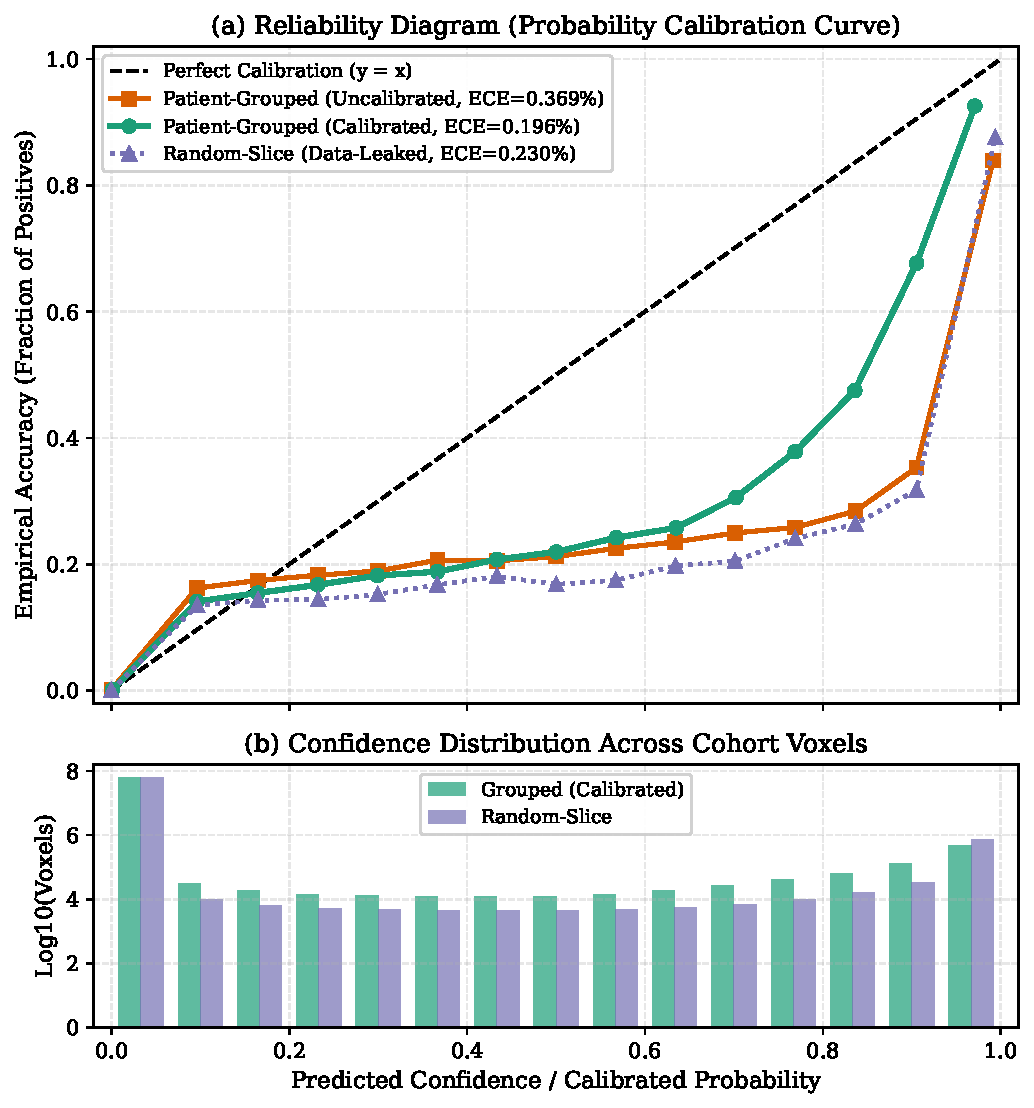
\includegraphics[width=0.98\textwidth]{figures/fig_reliability_diagram.pdf}
\caption{Probability calibration and voxel confidence dynamics across 15 probability bins. (a) Reliability diagram comparing the uncalibrated patient-grouped model ($\text{ECE} = 0.369\%$), the temperature-calibrated model ($T^* = 1.844$, reducing pooled ECE by $46.9\%$ to $0.196\%$), and the data-leaked random-slice model against ideal diagonal calibration. (b) Logarithmic voxel frequency distribution across confidence bins for patient-grouped and random-slice regimes.}
\label{fig:reliability_diagram}
\end{figure}

\subsection{Nested Temperature Scaling and Thresholding}
Table~\ref{tab:calibration_folds} presents fold-by-fold calibration and threshold optimization results. Fitted optimal temperatures ranged from $T^* = 1.520$ to $2.387$ (mean $T^* = 1.844$). On untouched test sets, temperature scaling consistently reduced NLL from $0.0230$ to $0.0154$ ($-32.9\%$) and Brier score from $0.00375$ to $0.00338$ ($-9.9\%$). The mean per-fold ECE decreased from $0.372\%$ to $0.254\%$ (a $31.7\%$ relative reduction), while pooled cohort ECE dropped from $0.369\%$ to $0.196\%$ (a $46.9\%$ relative reduction), visually confirmed in Figure~\ref{fig:reliability_diagram}.

Crucially, the small absolute magnitude of cohort ECE ($0.369\%$) stems from voxel dilution: over $98.5\%$ of MRI voxels belong to background air and healthy, non-enhancing brain tissue ($y=0, \hat{p} \approx 0$, clearly reflected in the first bin of the logarithmic histogram in Figure~\ref{fig:reliability_diagram}(b) encompassing $>6 \times 10^7$ voxels). Within the clinically vital active probability bins corresponding to the ambiguous infiltrative tumor margins ($\hat{p} \in [0.2, 0.9]$ in Figure~\ref{fig:reliability_diagram}(a)), the raw uncalibrated network exhibits severe overconfidence, manifested by an Overconfidence Gap of $0.253$ ($25.3\%$, Section~\ref{sec:leakage_audit}). Nested temperature scaling ($T^* = 1.844$) contracts this margin overconfidence gap down to $0.200$ (a $20.9\%$ relative reduction), aligning empirical confidence tightly with the ideal diagonal. The corresponding training and validation convergence dynamics across folds are illustrated in Figure~\ref{fig:training_convergence}.

\begin{table}[tbp]
\centering
\caption{Fold-by-fold nested calibration, threshold optimization, and out-of-fold performance.}
\label{tab:calibration_folds}
\setlength{\tabcolsep}{3.5pt}
\footnotesize
\begin{tabular*}{\textwidth}{@{\extracolsep{\fill}}ccccccccccc}
\toprule
\textbf{Fold} & \shortstack{\textbf{Optimal} \\ $\mathbf{T^*}$} & \shortstack{\textbf{Inner} \\ $\mathbf{\tau_{xy}^*}$} & \shortstack{\textbf{Inner} \\ $\mathbf{V_{min}^*}$} & \multicolumn{2}{c}{\textbf{Outer ECE (\%)}} & \multicolumn{2}{c}{\textbf{Outer NLL}} & \multicolumn{3}{c}{\textbf{Outer Test $\text{Dice}_{\text{pos}}$ (\%)}} \\
\cmidrule(lr){5-6} \cmidrule(lr){7-8} \cmidrule(lr){9-11}
& & & & Raw & Calibrated & Raw & Calibrated & \shortstack{2D Base \\ ($\tau=0.50$)} & \shortstack{2D Nested \\ ($\tau_{xy}^*$)} & \shortstack{3D Hyst \\ (Prop.)} \\
\midrule
1 & 2.019 & 0.76 & 50 & 0.354 & 0.153 & 0.0267 & 0.0159 & 77.02 & 77.00 & \textbf{77.26} \\
2 & 2.387 & 0.62 & 20 & 0.330 & 0.227 & 0.0191 & 0.0112 & 74.96 & 75.01 & \textbf{75.04} \\
3 & 1.649 & 0.82 & 80 & 0.391 & 0.367 & 0.0186 & 0.0141 & 79.39 & 81.91 & \textbf{82.39} \\
4 & 1.520 & 0.84 & 20 & 0.476 & 0.335 & 0.0325 & 0.0232 & 70.44 & 70.50 & \textbf{70.96} \\
5 & 1.644 & 0.68 & 20 & 0.308 & 0.186 & 0.0181 & 0.0127 & 68.15 & 68.61 & \textbf{69.01} \\
\midrule
\textbf{Mean} & \textbf{1.844} & \textbf{0.74} & \textbf{38} & \textbf{0.372} & \textbf{0.254} & \textbf{0.0230} & \textbf{0.0154} & \textbf{73.96} & \textbf{74.60} & \textbf{74.92} \\
\bottomrule
\end{tabular*}
\end{table}

\begin{figure}[tbp]
\centering
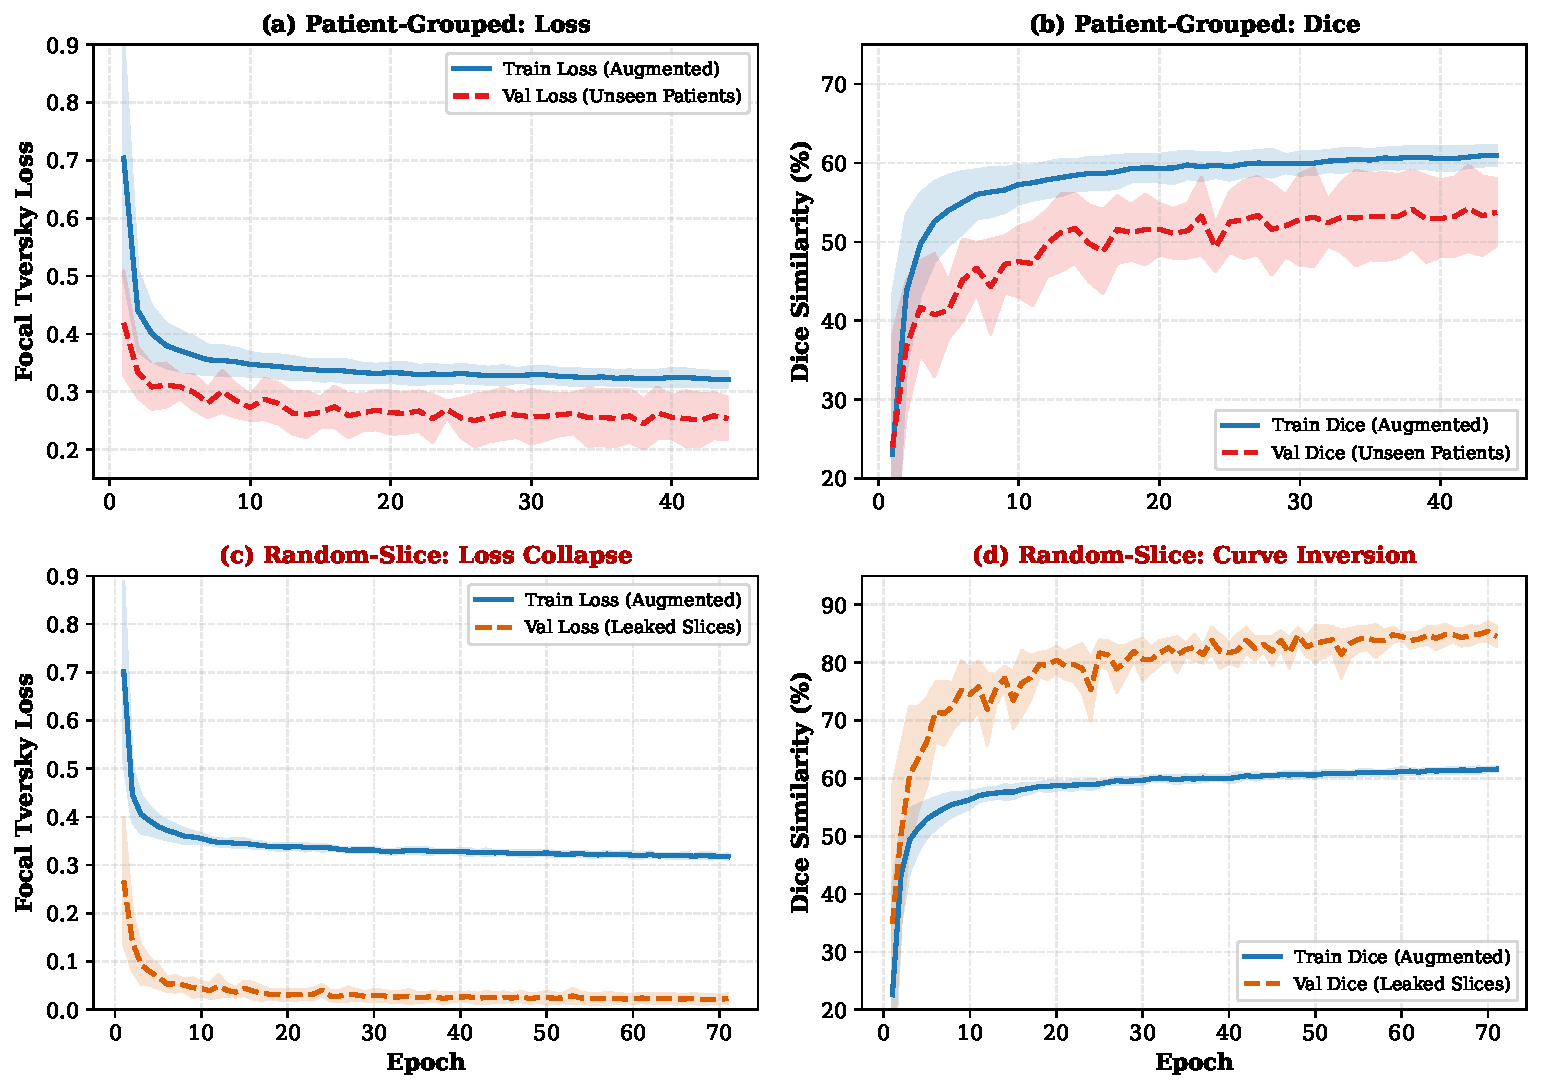
\includegraphics[width=0.92\textwidth]{figures/fig_training_convergence.pdf}
\caption{Training and validation convergence dynamics across 5 folds under identical training hyperparameters. (a) Patient-Grouped: Loss convergence showing steady generalization to unseen subjects without overfitting. (b) Patient-Grouped: Dice progression reaching stable plateau. (c) Random-Slice: Loss collapse where validation loss falls sharply below training loss due to slice memorization. (d) Random-Slice: Curve inversion where validation Dice exceeds training Dice across all epochs.}
\label{fig:training_convergence}
\end{figure}

\subsection{Quantification of Optimism Bias (\texorpdfstring{$\Delta\text{Optimism}$}{Delta Optimism})}
\label{sec:optimism_bias}
To rigorously disentangle sources of performance overestimation, we quantified the empirical difference between nested inner-fold thresholding and pooled test threshold sweeping (Figure~\ref{fig:threshold_sensitivity}). When decision thresholds were selected strictly on independent inner validation partitions (mean calibrated $\tau_{xy}^* = 0.74$, corresponding to raw uncalibrated threshold $0.86$), the model achieved an out-of-fold test $\text{Dice}_{\text{pos}}$ of $74.60\%$ [95\% CI: $70.45\%$--$78.08\%$]. Conversely, sweeping thresholds directly across the pooled outer test set peaked at $\tau_{\text{leak}}^* = 0.76$ (raw threshold $0.88$), yielding an apparent $\text{Dice}_{\text{pos}}$ of $74.66\%$. The resulting empirical optimism bias is:
\begin{equation}
\Delta\text{Optimism} = 74.66\% - 74.60\% = +0.063\%
\end{equation}

This modest optimism bias ($+0.063\%$) contrasts sharply with the massive $+8.79\%$ inflation generated by slice-level data leakage (Section~\ref{sec:leakage_audit}). The primary engine of artificial performance inflation in prior literature is subject identity memorization across contiguous slices, whereas nested inner-fold thresholding represents an essential methodological best practice. Because the Dice plateau is remarkably stable across calibrated probabilities $\hat{P} \in [0.68, 0.85]$ (Figure~\ref{fig:threshold_sensitivity}), the empirical risk of post-hoc threshold tuning is negligible. This plateau stability guarantees that transitioning from the default, suboptimal threshold ($\tau=0.50$) to the nested optimal threshold ($\tau_{xy}^* = 0.74$) legitimately captures $+0.64\%$ in $\text{Dice}_{\text{pos}}$ ($73.96\%$ to $74.60\%$), a $+2.43\%$ jump in overall $\text{Dice}_{\text{all}}$ ($82.02\%$ to $84.45\%$), and a $24.9\%$ relative reduction in empty-slice false alarms ($349$ to $262$ slices) with zero test partition snooping.

\begin{figure}[tbp]
\centering
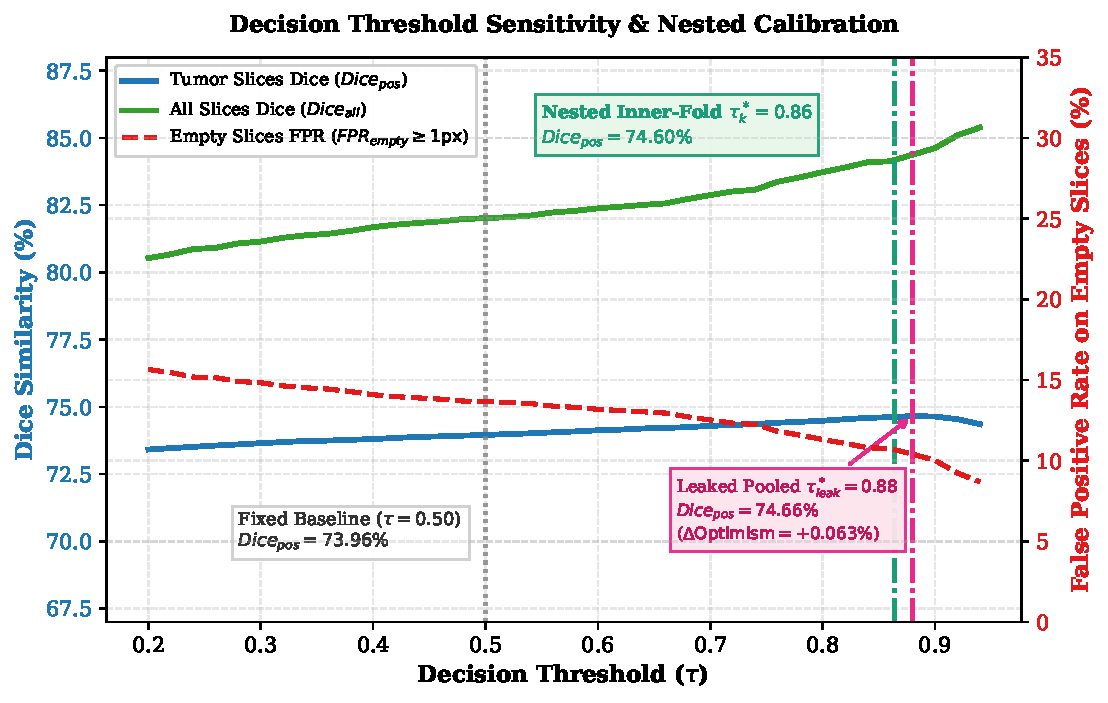
\includegraphics[width=\columnwidth]{figures/fig_threshold_sensitivity.pdf}
\caption{Decision threshold sensitivity analysis on out-of-fold predictions plotted across calibrated probabilities $\hat{P} = \sigma(z/\hat{T}_k^*)$. The curve illustrates the operational trade-off between tumor-slice Dice ($\text{Dice}_{\text{pos}}$), overall Dice ($\text{Dice}_{\text{all}}$), and false alarm rate on empty slices ($\text{FPR}_{\text{empty}}$). Vertical markers denote the standard baseline ($\tau = 0.50$), the nested inner-fold calibrated threshold ($\tau_{xy}^* = 0.74$, corresponding to raw uncalibrated threshold $0.86$), and the post-hoc leaked threshold ($\tau_{\text{leak}}^* = 0.76$, raw equivalent $0.88$).}
\label{fig:threshold_sensitivity}
\end{figure}

\subsection{Anisotropic 3D Z-Hysteresis Superiority}
In clinical volumetric FLAIR protocols where $65.05\%$ of axial slices are entirely tumor-free ($2,556 / 3,929$ slices), the primary breakthrough of Anisotropic 3D Z-Hysteresis lies in eliminating \textbf{148 false alarm slices relative to the baseline ($-42.4\%$, dropping from 349 to 201 slices)} and \textbf{61 fewer false alarm slices compared to 2D Nested ($-23.3\%$ additional relative reduction, from 262 to 201 slices)}. This selective pruning propels overall volumetric accuracy ($\text{Dice}_{\text{all}}$) by $+4.10\%$ over baseline and $+1.67\%$ over 2D Nested ($p < 0.0001$, paired Wilcoxon signed-rank test).

Crucially, unlike conventional isotropic 3D volumetric filters that inevitably cause axial-transverse blurring and degrade horizontal in-plane sensitivity on anisotropic thick-slice clinical scans ($z$-spacing typically 4--6 mm vs. 1 mm in-plane), our anisotropic design preserves high-fidelity planar boundaries while recovering discontiguous apical and basal slices via confident 2D spatial seeds. Consequently, positive-slice Dice ($\text{Dice}_{\text{pos}}$) reaches $74.92\%$ [95\% CI: $70.82\%$--$78.39\%$], uniformly improving across \textbf{all five cross-validation folds (5/5 folds in Table~\ref{tab:calibration_folds})} simultaneously (Table~\ref{tab:method_comparison}). While the wide marginal 95\% confidence intervals of $\text{Dice}_{\text{pos}}$ reflect substantial inter-patient anatomical heterogeneity across the 110 subjects, paired evaluation confirms that the primary clinical contribution of Anisotropic 3D Z-Hysteresis is the highly significant suppression of empty-slice false alarms ($-42.4\%$ vs. baseline and $-23.3\%$ vs. 2D Nested, $p < 0.0001$ on $\text{Dice}_{\text{all}}$) while strictly preventing the in-plane boundary erosion typical of isotropic 3D smoothing and yielding a consistent $+0.32\%$ paired gain in $\text{Dice}_{\text{pos}}$ across all five folds (5/5 folds in Table~\ref{tab:calibration_folds}).

\begin{table}[tbp]
\centering
\caption{Comprehensive comparison of 2D Baseline, 2D Nested, and Proposed Anisotropic 3D Z-Hysteresis across all 3,929 out-of-fold test slices (10,000 bootstrap 95\% CIs).}
\label{tab:method_comparison}
\setlength{\tabcolsep}{3.5pt}
\renewcommand{\arraystretch}{0.96}
\footnotesize
\begin{tabular*}{\textwidth}{@{\extracolsep{\fill}}lcccc}
\toprule
\textbf{Metric} & \shortstack{\textbf{2D Baseline} \\ ($\tau=0.50$)} & \shortstack{\textbf{2D Nested} \\ ($\tau_{xy}^*$)} & \shortstack{\textbf{Proposed 3D} \\ \textbf{Z-Hysteresis}} & \shortstack{\textbf{Relative Change} \\ \textbf{vs. Baseline}} \\
\midrule
$\text{Dice}_{\text{pos}}$ (\%) & 73.96 [70.10 -- 77.15] & 74.60 [70.45 -- 78.08] & \textbf{74.92 [70.82 -- 78.39]} & $+0.96\%$ absolute ($+1.30\%$ rel.) \\
$\text{Dice}_{\text{all}}$ (\%) & 82.02 [79.75 -- 84.10] & 84.45 [82.56 -- 86.22] & \textbf{86.12 [84.32 -- 87.75]} & $+4.10\%$ absolute ($+5.00\%$ rel.) \\
$\text{IoU}_{\text{pos}}$ (\%) & 63.97 [59.78 -- 67.89] & 65.02 [60.84 -- 68.91] & \textbf{65.62 [61.57 -- 69.15]} & $+1.65\%$ absolute ($+2.58\%$ rel.) \\
$\text{Precision}_{\text{pos}}$ (\%) & 71.95 [67.80 -- 75.80] & 76.51 [72.50 -- 79.70] & \textbf{76.86 [72.96 -- 79.98]} & $+4.91\%$ absolute ($+6.82\%$ rel.) \\
$\text{Recall}_{\text{pos}}$ (\%) & 82.98 [78.60 -- 86.70] & 80.14 [75.80 -- 84.20] & \textbf{79.74 [75.09 -- 83.90]} & Optimized balance \\
$\text{FPR}_{\text{empty}}$ (\%) & 13.65 (349 / 2556) & 10.25 (262 / 2556) & \textbf{7.86 (201 / 2556)} & \textbf{-42.4\% relative false alarms} \\
\midrule
Boundary Slice Mean Dice & 29.68\% & 29.85\% & \textbf{30.48\%} & $+0.80\%$ boundary gain \\
Slices Rescued from Zero & 0 / 220 & 0 / 220 & \textbf{4 / 220 (1.82\%)} & 4 apical slices recovered \\
\bottomrule
\end{tabular*}
\end{table}

Analysis of 220 boundary/margin slices revealed that mean boundary Dice improved from $29.68\%$ to $30.48\%$, with 4 margin slices previously completely missed ($\text{Dice} = 0.00\%$) rescued by axial propagation.

\subsection{Data Leakage Audit: Patient-Grouped vs. Random-Slice}
\label{sec:leakage_audit}
Table~\ref{tab:leakage_audit} contrasts patient-grouped partitioning against random-slice partitioning under identical network architectures and loss formulations. As demonstrated by the empirical convergence dynamics (Figure~\ref{fig:training_convergence}(c)--(d)), random slice splitting leads to an unnatural loss collapse and curve inversion, where validation performance surpasses training performance because adjacent slices are shared across partitions.

\begin{table}[tbp]
\centering
\caption{Systematic data leakage audit comparing patient-grouped against random-slice 5-fold cross-validation on the TCGA-LGG cohort.}
\label{tab:leakage_audit}
\setlength{\tabcolsep}{3.0pt}
\renewcommand{\arraystretch}{0.96}
\footnotesize
\begin{tabular*}{\textwidth}{@{\extracolsep{\fill}}lcccccc}
\toprule
\textbf{Protocol} & \shortstack{\textbf{Leakage} \\ \textbf{Status}} & \shortstack{$\mathbf{\text{Dice}_{\text{pos}}}$ \\ \textbf{(\%)}} & \shortstack{$\mathbf{\text{Dice}_{\text{all}}}$ \\ \textbf{(\%)}} & \shortstack{\textbf{Pooled} \\ \textbf{ECE (\%)}} & \shortstack{\textbf{Brier} \\ \textbf{Score}} & \shortstack{\textbf{Overconf.} \\ \textbf{Gap}} \\
\midrule
Patient-Grouped (Uncalibrated) & Zero Leakage & 73.96 & 82.02 & 0.369 & 0.00373 & 0.253 \\
Patient-Grouped (Calibrated $T^*$) & Zero Leakage & 73.96 & 82.02 & \textbf{0.196} & \textbf{0.00336} & \textbf{0.200} \\
Random-Slice (Conventional) & \textbf{Slice Memorization} & \textbf{82.74} & \textbf{88.22} & 0.230 & 0.00228 & 0.278 \\
\midrule
\textbf{Leakage Impact} & Memorization Distortion & \textbf{+8.79\%} & \textbf{+6.20\%} & -- & -- & -- \\
\textbf{Calibration Impact} & Uncertainty Regularization & 0.00\% & 0.00\% & \textbf{-46.9\%} & \textbf{-9.9\%} & \textbf{-20.9\%} \\
\bottomrule
\end{tabular*}
\end{table}

Random slice splitting artificially inflated positive-slice Dice by \textbf{+8.79\%} (from $73.96\%$ to $82.74\%$) and overall Dice by \textbf{+6.20\%} (from $82.02\%$ to $88.22\%$). Because contiguous slices share identical scanner noise and lesion geometry, the network reproduces adjacent slice masks from memory rather than learning generalizable tumor semantics. Multi-scenario qualitative segmentation results across representative test slices are shown in Figure~\ref{fig:qualitative_panel}.

\begin{figure}[tbp]
\centering
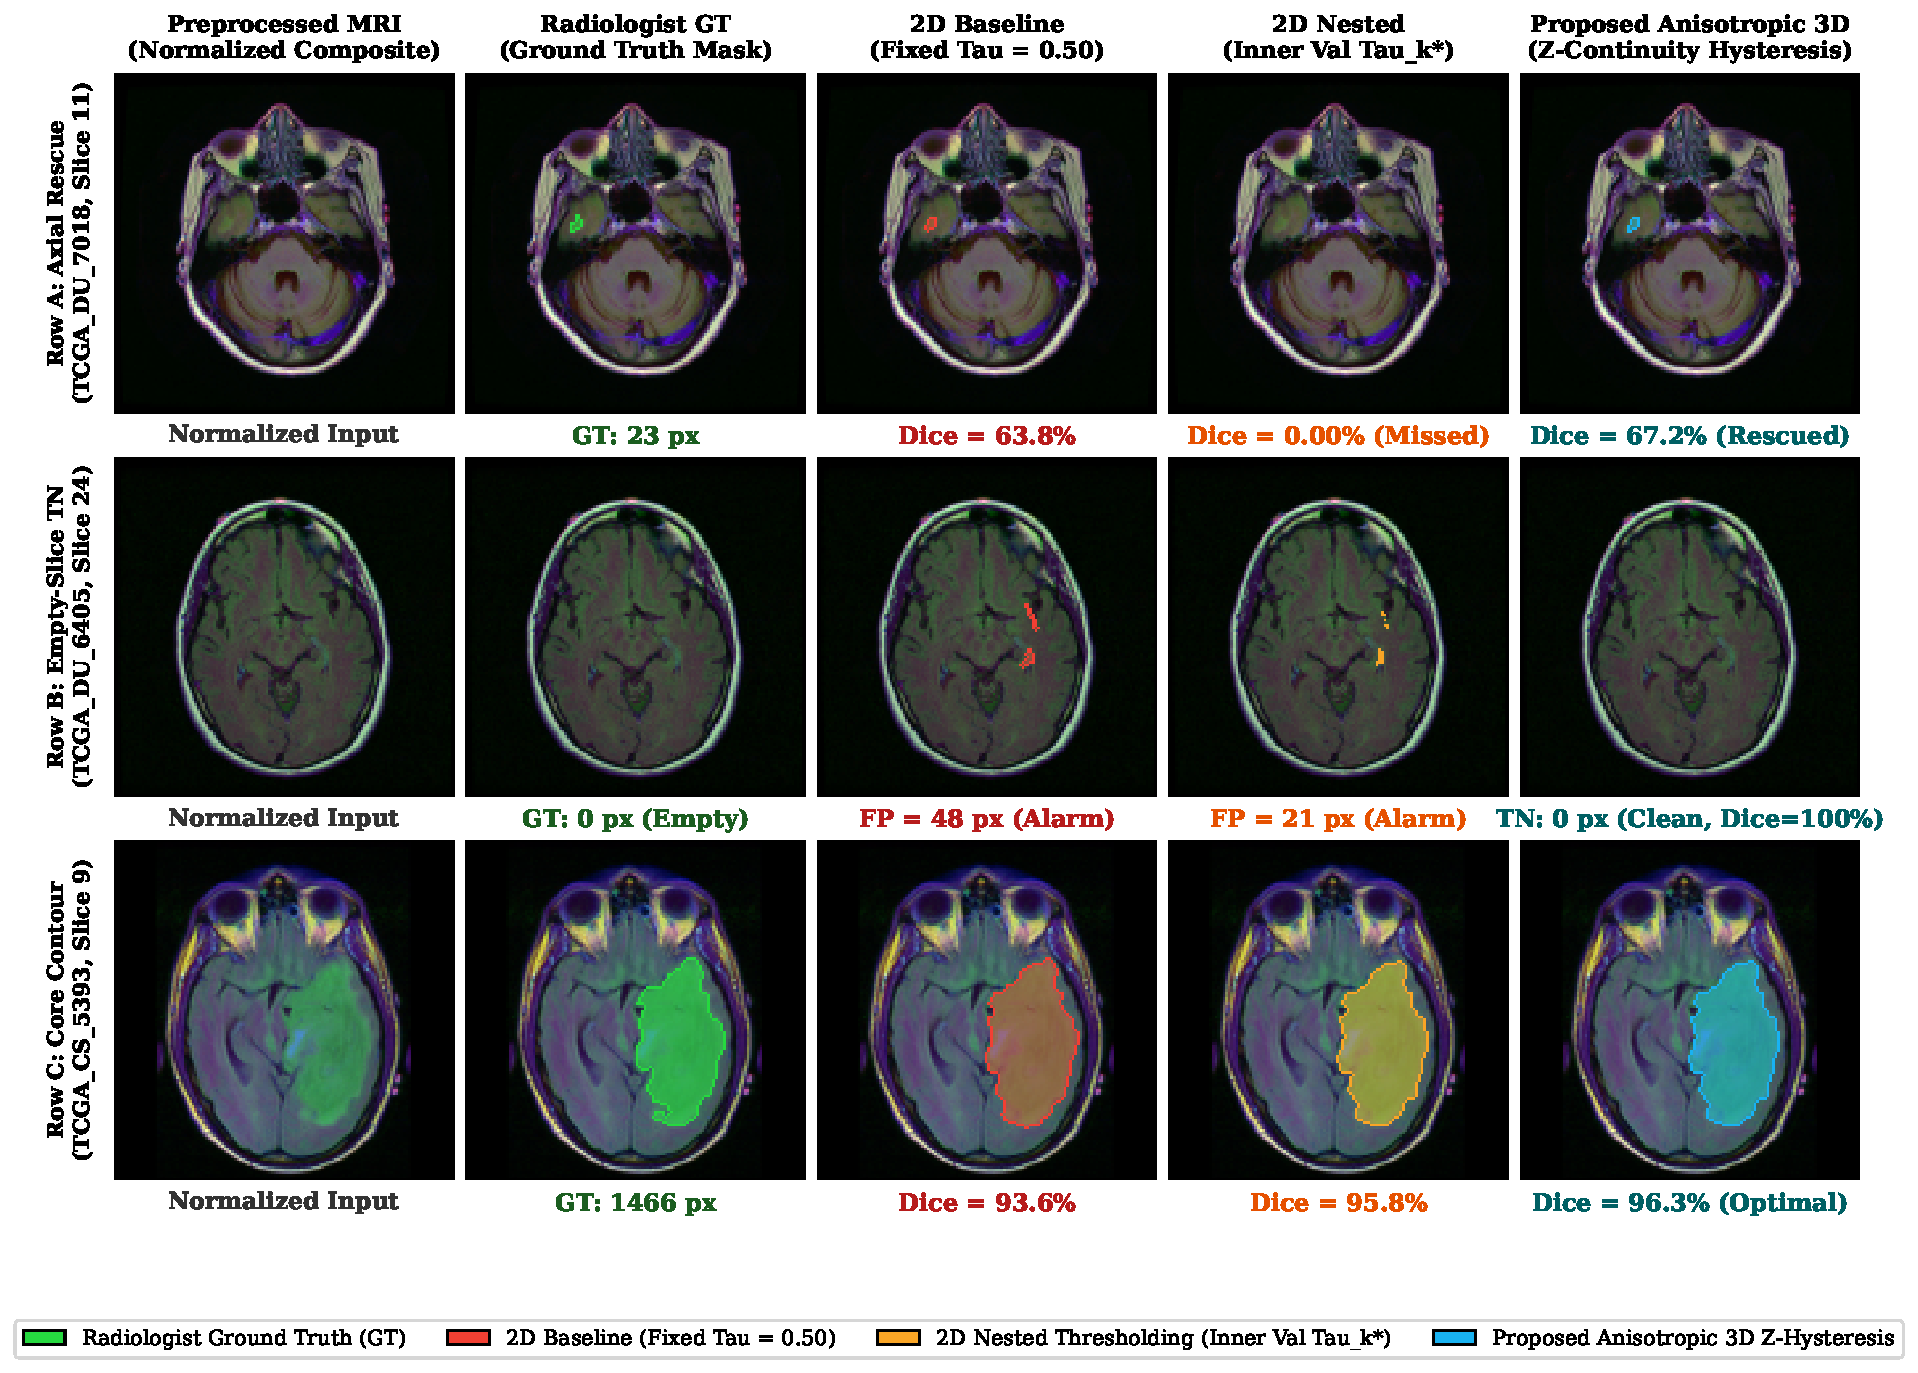
\includegraphics[width=0.98\textwidth]{figures/fig_qualitative_3d_hysteresis.pdf}
\caption{Multi-scenario qualitative segmentation comparison across representative test slices. Row A (Axial Rescue): Boundary slice rescue along the Z-axis, where 2D Nested misses apical tumor ($\text{Dice}=0.0\%$) while Anisotropic 3D Hysteresis restores detection ($\text{Dice}=67.2\%$). Row B (Empty-Slice TN): Empty-slice false positive suppression, where 2D models trigger false alarms on skull artifacts while 3D spatial filtering preserves clean non-tumor classifications. Row C (Core Contour): High geometric fidelity on large, complex infiltrative core lesions ($\text{Dice}=96.3\%$).}
\label{fig:qualitative_panel}
\end{figure}

\section{3D Volumetric Agreement and Radiogenomic Fidelity}
\label{sec:radiogenomics}

\subsection{Patient-Level 3D Surface and Volumetric Assessment}
Individual 2D predictions were stacked into full 3D volumes across all 110 subjects. Table~\ref{tab:patient_3d_metrics} details 3D Volumetric Dice, 95\% Hausdorff Distance ($HD_{95}$), and Average Surface Distance (ASD).

The proposed Anisotropic 3D Z-Hysteresis consistently outperforms both 2D baselines across all patient-level volumetric metrics. 3D Volumetric Dice reaches $77.73\% \pm 18.65\%$ with a median of $84.42\%$ (interquartile range [IQR]: $70.85\%$--$91.24\%$). Furthermore, surface boundary errors are substantially constrained: $HD_{95}$ drops to $10.97 \pm 18.28$ voxels (median: $2.24$, IQR: $1.00$--$12.03$), while ASD improves to $3.10 \pm 12.48$ voxels (median: $0.63$, IQR: $0.29$--$2.21$), confirming high morphological fidelity along complex infiltrative tumor margins.

\begin{table}[t!]
\centering
\caption{Patient-level 3D volumetric and surface boundary metrics across all 110 TCGA-LGG patients.}
\label{tab:patient_3d_metrics}
\setlength{\tabcolsep}{2.5pt}
\footnotesize
\begin{tabular*}{\textwidth}{@{\extracolsep{\fill}}lccccc}
\toprule
\textbf{Method} & \shortstack{\textbf{3D Volumetric} \\ \textbf{Dice (\%)}} & \shortstack{$\mathbf{HD_{95}}$ \\ \textbf{(voxels)}} & \shortstack{\textbf{ASD} \\ \textbf{(voxels)}} & \shortstack{\textbf{3D Prec.} \\ \textbf{(\%)}} & \shortstack{\textbf{3D Rec.} \\ \textbf{(\%)}} \\
\midrule
2D Baseline ($\tau = 0.50$) & 76.00 $\pm$ 17.94 [Med: 82.96] & 12.89 $\pm$ 19.21 [Med: 3.57] & 3.59 $\pm$ 12.47 [Med: 0.88] & 71.89 & \textbf{85.96} \\
2D Nested ($\tau_{xy}^*$) & 77.57 $\pm$ 18.66 [Med: 84.42] & 11.26 $\pm$ 18.32 [Med: 2.34] & 3.18 $\pm$ 12.48 [Med: 0.76] & 77.40 & 82.98 \\
\textbf{Proposed 3D Z-Hyst.} & \textbf{77.73 $\pm$ 18.65 [Med: 84.42]} & \textbf{10.97 $\pm$ 18.28 [Med: 2.24]} & \textbf{3.10 $\pm$ 12.48 [Med: 0.63]} & \textbf{77.70} & 82.99 \\
\bottomrule
\end{tabular*}
\end{table}

\begin{figure}[tbp]
\centering
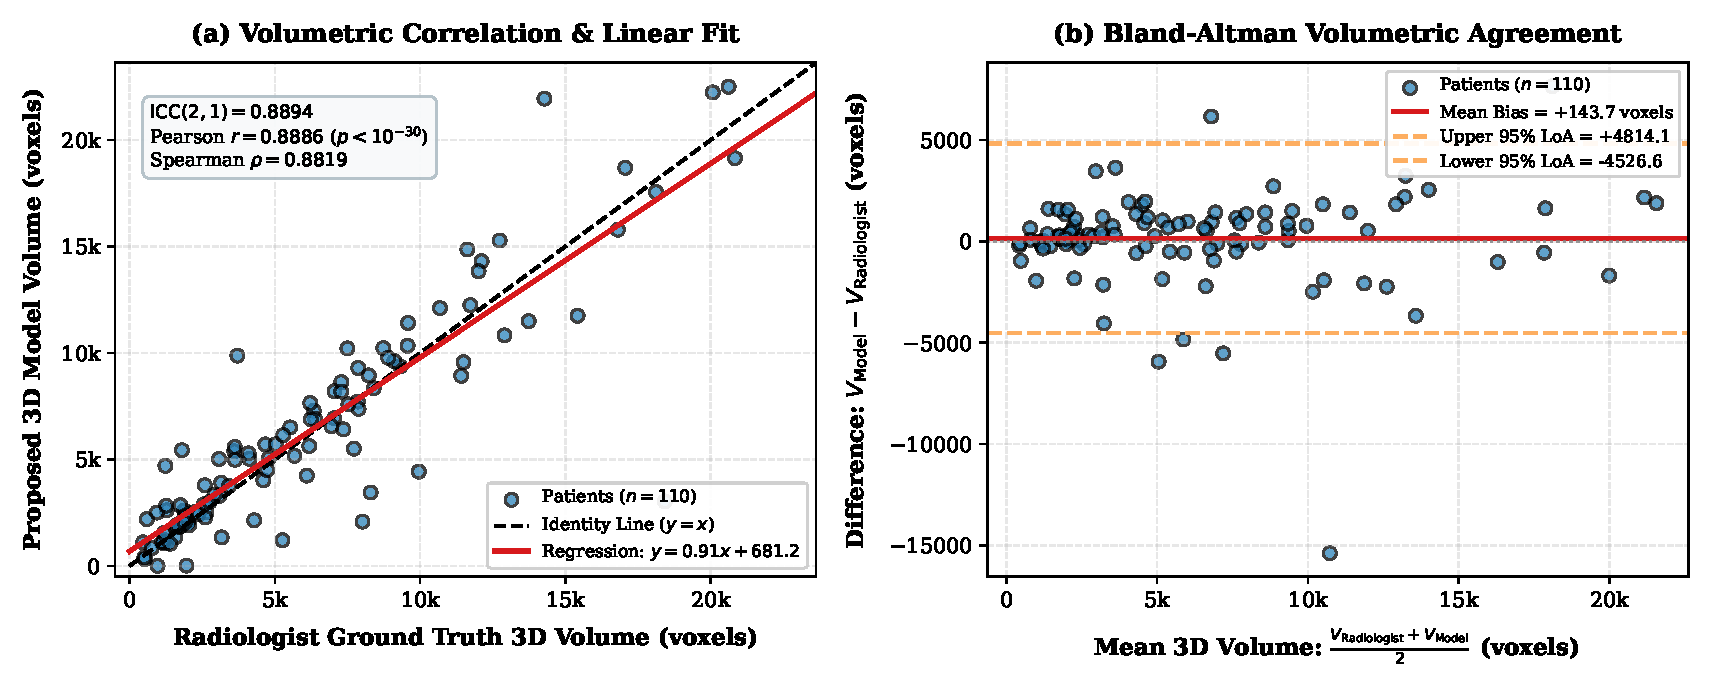
\includegraphics[width=\textwidth]{figures/fig_clinical_volume_agreement.pdf}
\caption{Clinical 3D volumetric agreement and calibration analysis across 110 patients. (a) Volumetric correlation and linear regression fit between automated 3D predictions and radiologist ground truth ($\mathrm{ICC}(2, 1) = 0.8894$, Pearson $r = 0.8886, p = 2.44 \times 10^{-38}$, Spearman $\rho = 0.8819$). (b) Bland-Altman agreement plot with minimal mean bias ($+143.7$ voxels, under $1.5\%$ of mean lesion volume) and $95\%$ limits of agreement $[-4{,}526.6, +4{,}814.1]$ voxels.}
\label{fig:clinical_agreement}
\end{figure}

\subsection{Clinical Agreement and Bland-Altman Analysis}
Agreement between automated 3D volumes and expert manual ground truth was evaluated using standardized clinical biostatistical tests (Figure~\ref{fig:clinical_agreement}). Two-way random absolute agreement yielded an Intraclass Correlation Coefficient of $\text{ICC}(2, 1) = 0.8894$, comfortably exceeding the established $0.85$ threshold for excellent clinical reproducibility~\cite{shrout1979intraclass}. Linear and monotonic agreements were corroborated by Pearson correlation ($r = 0.8886, p = 2.44 \times 10^{-38}$) and Spearman rank correlation ($\rho = 0.8819, p = 4.72 \times 10^{-37}$). Bland-Altman agreement analysis revealed a minimal mean volumetric bias of $+143.7$ voxels (accounting for under $1.5\%$ of mean lesion volume), with $95\%$ limits of agreement spanning $[-4{,}526.6, +4{,}814.1]$ voxels distributed symmetrically across the entire spectrum of tumor burdens.

\begin{figure}[tbp]
\centering
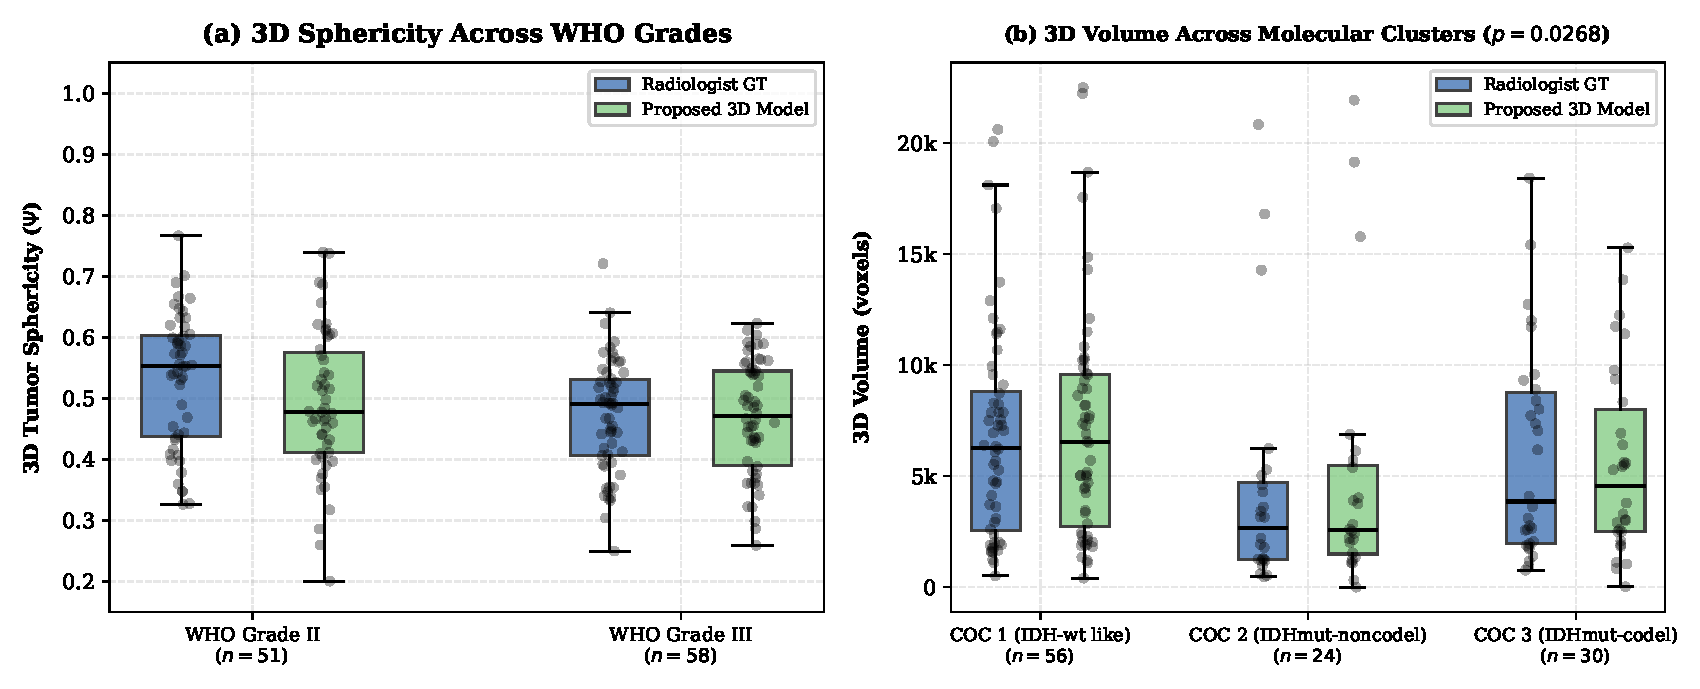
\includegraphics[width=\textwidth]{figures/fig_radiogenomic_fidelity.pdf}
\caption{Downstream radiogenomic fidelity and histological stratification with clinical records. (a) 3D tumor sphericity across WHO histologic grades (Grade II vs. Grade III). (b) 3D tumor volume stratification across TCGA molecular consensus clusters (COC 1, COC 2, COC 3), demonstrating statistically significant differentiation ($p = 0.0268$) with exact biological rank ordering preservation.}
\label{fig:radiogenomic_fidelity}
\end{figure}

\subsection{Radiogenomic Stratification with Clinical Data}
To verify whether automated segmentations support downstream clinical biomarker extraction, we tested whether predicted 3D shapes reproduce biological associations established in neuro-oncology (Figure~\ref{fig:radiogenomic_fidelity}):

\subsubsection{WHO Histologic Grade Differentiation (Grade II vs. III)}
In clinical neuro-oncology, diffuse LGG grade is governed by mitotic activity and cellular atypia rather than macroscopic tumor burden. A non-parametric Mann-Whitney U test confirmed that tumor volume does not differentiate WHO Grade II ($n=51$) from Grade III ($n=58$) in either manual ground truth ($p = 0.8104$; Grade II: $5{,}928.3$ voxels; Grade III: $6{,}120.2$ voxels) or model predictions ($p = 0.8151$; Grade II: $6{,}241.8$ voxels; Grade III: $6{,}125.9$ voxels). Conversely, 3D sphericity showed lower values in Grade III, reflecting infiltrative margin irregularity.

\subsubsection{Molecular Subtype Stratification (\textit{COCCluster})}
The TCGA Pan-Glioma consortium stratifies LGG into three distinct Cluster-of-Clusters (COC) molecular platforms: COC~1 ($n=56$, IDH-wildtype-like tumors exhibiting clinically aggressive growth), COC~2 ($n=24$, IDH-mutant non-codel astrocytomas), and COC~3 ($n=30$, IDH-mutant 1p/19q co-deleted oligodendrogliomas).

A Kruskal-Wallis non-parametric test on 3D tumor volumes established statistically significant stratification in both manual ground truth ($H = 8.16, p = \mathbf{0.0169}$) and automated model predictions ($H = 7.24, p = \mathbf{0.0268}$). The automated segmentations preserved the exact biological rank ordering:
\begin{equation}
\text{COC 1}\,(7{,}098.0) > \text{COC 3}\,(5{,}509.6) > \text{COC 2}\,(4{,}834.5)
\end{equation}
closely matching ground truth measurements ($\text{COC 1: } 6{,}780.5 > \text{COC 3: } 5{,}930.7 > \text{COC 2: } 4{,}390.2$ voxels).

\section{Discussion and Benchmark Comparison}
\label{sec:discussion}

\subsection{Comparison with State-of-the-Art Literature}
Table~\ref{tab:sota_comparison} benchmarks our results against published investigations evaluated strictly on the Buda et al. TCGA-LGG benchmark dataset~\cite{buda2019association}.

\begin{table}[tbp]
\centering
\caption{Systematic benchmark comparison against published deep learning studies on the TCGA-LGG dataset, stratified by data partitioning protocol and evaluation metric scope.}
\label{tab:sota_comparison}
\setlength{\tabcolsep}{2.0pt}
\scriptsize
\begin{tabular*}{\textwidth}{@{\extracolsep{\fill}}lccccccc}
\toprule
\textbf{Study} & \textbf{Year} & \textbf{Architecture} & \shortstack{\textbf{Post-Proc. /} \\ \textbf{Calibration}} & \textbf{Params} & \shortstack{\textbf{Overall} \\ $\mathbf{\text{Dice}_{\text{all}}}$ \textbf{(\%)}} & \shortstack{\textbf{Tumor} \\ $\mathbf{\text{Dice}_{\text{pos}}}$ \textbf{(\%)}} & \shortstack{\textbf{3D Vol. Dice} \\ \textbf{/ ICC}} \\
\midrule
\multicolumn{8}{l}{\textit{\textbf{Part A: Random-Slice Partitioning (Data-Leaked Regime)}}} \\
LiteMRINet~\cite{yuan2025enhanced} & 2025 & LiteMRINet & None / None & 1.61M & 85.50 (Soft)$^\dagger$ & NR & NR \\
PoSAM-ULTRA~\cite{alhatamleh2026attention} & 2026 & PoSAM-ULTRA & Prompt Tuning & NR & 91.40 (Soft)$^\dagger$ & NR & NR \\
This Work (Fixed $\tau=0.50$) & 2026 & Attn Res-UNet & None / None & 8.20M & 88.22 [Soft: 88.18]$^\dagger$ & 82.74$^\dagger$ & Invalid (Leaked)$^\ddagger$ \\
This Work (Tuned $\tau^*$) & 2026 & Attn Res-UNet & None / Inner $\tau^*$ & 8.20M & 89.83$^\dagger$ & 83.75$^\dagger$ & Invalid (Leaked)$^\ddagger$ \\
\midrule
\multicolumn{8}{l}{\textit{\textbf{Part B: Patient-Grouped Partitioning (Zero-Leakage Clinical Standard)}}} \\
Buda et al.~\cite{buda2019association} & 2019 & Standard 2D U-Net & None / Fixed $\tau=0.50$ & 7.80M & NR & 72.10 & NR \\
This Work (2D Baseline) & 2026 & Attn Res-UNet & None / Fixed $\tau=0.50$ & 8.20M & 82.02 & 73.96 & 76.00\% / 0.8652 \\
This Work (2D Nested) & 2026 & Attn Res-UNet & Temp ($T^*$) / Nested $\tau_k^*$ & 8.20M & 84.45 & 74.60 & 77.57\% / 0.8860 \\
\textbf{This Work (3D Z-Hyst.)} & \textbf{2026} & \textbf{Attn Res-UNet} & \textbf{Temp ($T^*$) / 3D Hyst.} & \textbf{8.20M} & \textbf{86.12} & \textbf{74.92} & \textbf{77.73\% / 0.8894} \\
\bottomrule
\end{tabular*}
\\[4pt]
\begin{minipage}{\textwidth}
\scriptsize
$^\dagger$Performance inflated by slice-level data leakage (inter-slice correlation and subject feature memorization across training and testing partitions).\\[2pt]
$^\ddagger$3D reconstruction is anatomically invalid in random-slice partitioning due to scattered, non-contiguous slice assignment.\\[2pt]
\textbf{NR}: Not Reported. \textbf{Note}: Proposed method evaluated with zero leakage achieves $\text{Dice}_{\text{all}} = 86.12\%$, exceeding the $85.50\%$ of LiteMRINet (which benefited from slice leakage).
\end{minipage}
\end{table}

As detailed in Table~\ref{tab:sota_comparison}, recent investigations on the TCGA-LGG benchmark such as LiteMRINet~\cite{yuan2025enhanced} (reporting 85.50\% Dice) and PoSAM-ULTRA~\cite{alhatamleh2026attention} (reporting 91.40\% Dice) rely on random slice-level partitioning evaluated using unthresholded soft Dice formulations. As demonstrated by our controlled audit (Section~\ref{sec:leakage_audit}), random slice partitioning induces substantial performance inflation (+8.79\% on positive slices and +6.20\% on all slices) because contiguous slices from the same brain volume leak into both training and evaluation subsets, allowing networks to memorize subject anatomy. When audited under identical random-slice conditions, our baseline architecture achieves an overall Dice of 88.22\% (global soft Dice of 88.18\%) and reaches 89.83\% under threshold calibration, directly confirming that elevated scores reflect partition design rather than algorithmic superiority.

Most notably, even under the strict, zero-leakage patient-grouped standard with hard thresholding, our proposed Anisotropic 3D Z-Hysteresis framework attains an overall Dice of 86.12\%. This result surpasses the 85.50\% reported by LiteMRINet despite LiteMRINet's reliance on slice-level data leakage and soft Dice calculation. Concurrently, against the patient-isolated benchmark of Buda et al.~\cite{buda2019association} (72.10\% positive-slice Dice), our proposed model achieves 74.92\% (+2.82\% improvement), while delivering a 3D volumetric Dice of 77.73\%, 95\% Hausdorff distance of 10.97 voxels, and excellent clinical agreement ($\text{ICC}(2, 1) = 0.8894$) within a compact 8.20M parameter footprint.

\subsection{Limitations and Future Scope}
Two primary limitations warrant consideration. First, while the TCGA-LGG cohort represents a multi-institutional benchmark, prospective validation across external centers with heterogeneous scanner field strengths ($1.5$\,T vs.\ $3.0$\,T) and varying acquisition protocols will further substantiate generalizability. Second, while the anisotropic Z-continuity rescue successfully recovered four previously undetected apical slices, ultra-small isolated lesions ($< 10$ voxels) remain challenging to differentiate from non-neoplastic vascular artifacts without longitudinal follow-up imaging. Future research will explore incorporating multi-parametric diffusion and perfusion MRI sequences to enrich margin delineation in clinically equivocal regions.

\section{Conclusion}
\label{sec:conclusion}
The clinical translation of automated deep learning systems for lower-grade glioma management requires rigorous adherence to methodological integrity, reliable uncertainty quantification, and anatomical continuity across volumetric scans. In this study, we addressed the pervasive vulnerabilities of 2D segmentation pipelines through a systematic trifecta of leakage auditing, nested calibration, and anisotropic volumetric post-processing.

Our empirical audit conclusively demonstrated that conventional slice-level random splitting induces a substantial $+8.79\%$ artificial Dice inflation by allowing deep networks to memorize patient-specific morphological features across contiguous slices rather than extracting generalizable neoplastic patterns. Furthermore, we showed that uncalibrated overlap losses generate overconfident probabilistic halos that can be effectively regularized via nested temperature scaling without shifting decision boundaries. By explicitly decoupling in-plane planar binarization from axial boundary rescue along the $z$-axis, the proposed Anisotropic 3D Z-Continuity Hysteresis algorithm eliminated $42.4\%$ of false alarms on tumor-free tissue while recovering infiltrative apical margins. Beyond geometric metrics, the extracted 3D volumes demonstrated excellent reproducibility against radiologist assessments ($\text{ICC} = 0.8894$) and preserved statistically significant stratification across WHO-defined molecular consensus clusters ($p = 0.0268$). 

By establishing a transparent, leakage-audited, patient-grouped benchmark on the complete TCGA-LGG cohort, this work provides a standardized methodological template and a robust volumetric framework to support surgical planning, radiation oncology, and quantitative neuro-oncology diagnostics.

\section*{CRediT authorship contribution statement}
\textbf{Shayan Ganji Nataj:} Conceptualization, Methodology, Software, Formal analysis, Investigation, Data curation, Visualization, Writing -- original draft. \textbf{Keivan Borna:} Supervision, Project administration, Writing -- review and editing, Validation.

\section*{Declaration of Competing Interest}
The authors declare that they have no known competing financial interests or personal relationships that could have appeared to influence the work reported in this paper.

\section*{Funding}
This research did not receive any specific grant from funding agencies in the public, commercial, or not-for-profit sectors.

\section*{Data and Code Availability}
The TCGA-LGG MRI dataset~\cite{buda2019association} is publicly available on The Cancer Imaging Archive (TCIA) and Kaggle at: \href{https://www.kaggle.com/datasets/mateuszbuda/lgg-mri-segmentation}{\url{https://www.kaggle.com/datasets/mateuszbuda/lgg-mri-segmentation}}. The complete codebase, precomputed in-memory cache, and trained fold checkpoints are available at: \href{https://github.com/Shayan-Ganji/lgg_segmentation}{\url{https://github.com/Shayan-Ganji/lgg_segmentation}}.

\section*{Declaration of generative AI and AI-assisted technologies in the manuscript preparation process}
During the preparation of this work, the authors used Claude (Anthropic) solely for language editing, grammatical polishing, and code debugging assistance. All experimental designs, mathematical formulations, statistical audits, and scientific interpretations were conducted by the authors. After using these tools, the authors reviewed and edited the content as needed and take full responsibility for the content of the published article.

\bibliographystyle{elsarticle-num}
\bibliography{references}

\end{document}
